\chapter*{Acknowledgements} \addcontentsline{toc}{chapter}{Acknowledgements}
\paragraph*{}
First of all, I am very grateful to Frédéric Thevenon for giving me the opportunity to work on such an exciting topic. I also thank him for his trust and support throughout my internship. Many thanks to Chady Zaza and Jeff Beisheim from the MAPDL solver team for their collaboration and technical help.

\paragraph*{}
I would also like to thank Florent Lopez, Guillaume Buron and Anthony Giacoma for the invaluable advice they gave me, as well as for the interesting conversations we had during these six months.

\paragraph*{}
Finally, I thank my internship supervisor, Jean-Charles Créput, for his responsiveness and for answering all my questions.

\chapter*{Introduction} \addcontentsline{toc}{chapter}{Introduction}
\paragraph*{}
As part of my studies at the University of Technology of Belfort-Montbéliard, I completed my final internship at Ansys France in Villeurbanne, which focused on the GPU acceleration of an eigensolver.

\paragraph*{}
Solvers are computational tools or algorithm used to find numerical solution of equation or system of equations. In particular, eigensolver finds eigenvalues and eigenvectors of a matrix, which are crucial in many scientific and engineering applications.

\paragraph*{}
In recent years, GPUs have shown impressive capabilities in a variety of tasks, especially in scientific computing. The aim of this work is to identify computationally expensive operations and to test different algorithms and tools that could accelerate the solver using GPUs, while ensuring robust numerical results. 


\tableofcontents
\newpage

\listoffigures
\newpage

\listofalgorithms

\printglossaries
\newpage



\chapter{Company Overview}
\section{Ansys}
\paragraph*{}
Ansys is an American company based in Canonsburg, employing over 6000 people, with more than 600 in France spread across several sites. The company designs numerical simulation software sold to other businesses in various industries (aerospace, automotive, etc.) to simulate physical effects during product design. The numerous applications of this software have made Ansys a dominant player in the numerical simulation market, with many companies using their products. The main products of Ansys are:
\begin{itemize}
    \item Ansys Mechanical for numerical simulation in mechanics
    \item Fluent for fluid dynamics (acquired in 2006)
    \item Ansoft for electromagnetics (acquired in 2008)
\end{itemize}
There are, of course, other software applications for various purposes such as optics and material databases.

\section{MAPDL Solver Team}
\paragraph*{}
John A. Swanson founded Ansys in 1970. His first finite element solver, written in Fortran, enabled simulations in the field of structural mechanics. Since then, the company has expanded its portfolio of solvers and simulation applications across numerous domains. However, MAPDL, the original solver, remains one of the company's technological gems. It continues to evolve and expand its capabilities, thanks to an international development team.

\paragraph*{}
In Lyon, part of this solver team is responsible for certain functionalities: eigenvalue analysis, linear dynamics applications, acoustic applications, generic \acrshort{hpc} mathematical tools, and establishing a communication architecture around this solver.


\newpage

\chapter{Background}
\section{Notation}
\paragraph*{}
Throughout this work, we usually follow the following convention for notating linear
algebra:
\begin{itemize}
    \item The fields of real and complex numbers are denoted by $\mathbb{R}$ and $\mathbb{C}$, respectively.
    \item  Elements in $\mathbb{R}$ and $\mathbb{C}$, scalars, are denoted by lowercase letters, $a, b, c, ...$ or $\alpha, \beta, \gamma, ...$
    \item Vectors are denoted by boldface lowercase letters, $\mathbf{u}, \mathbf{v}, \mathbf{w}, ...$ or $\mathbf{x}, \mathbf{y}, \mathbf{z}, ...$
    \item Matrices are denoted by uppercase roman letters, $A, B, C, ...$
    \item A block matrix is a matrix that is defined using smaller matrices, called blocks.
    \begin{align*}
        A &= \begin{bmatrix}
                A_{1,1} & A_{1,2}\\
                A_{2,1} & A_{2,2}
            \end{bmatrix}
            %,where $A \in \mathbb{R}^{m\times n}$ and $A_i \in \mathbb{R}^{p\times s}
    \end{align*}
        
    \item To simplify complex indexing, we use the notation $1:j = \{1,2,...,j\}$, thus
        \begin{align*}
        A_{1:j,k} &=
            \begin{bmatrix}
               a_{1,k} \\
               a_{2,k} \\
               \vdots \\
               a_{j,k}
            \end{bmatrix}
        \text{denote the $k$-th column of $A$ of size $j$}
        \end{align*} 

\item Concerning Kyrlov methods, the resulting subspace matrices are denoted by caligraphic uppercase letters, whose subscript is denoting the subspace order, $\mathcal{Q}_k, \mathcal{K}_k, \mathcal{V}_k,...$
\item We write boldface $\mathbf{0}$ for a length $n$ column vector of zeros.
\end{itemize}

\paragraph*{}
We formulate all of the methods described in this report to be correct either in
real or in complex arithmetic, using a single notation for both cases. We support this with
the following notation:

\begin{itemize}
    \item For a scalar $\alpha$, $\overline\alpha$ denotes its complex conjugate if $\alpha$ is complex, else $\overline\alpha$ = $\alpha$ if $\alpha$ is real.
    \item For a column vector $x$ of length $n$, $x^*$ denotes its transpose $(x^*=x^T)$ if $x$ is real, and its complex conjugate transpose $(x^*=\overline{x}^T)$ if $x$ is complex.
    \item Similarly, for an $m\times n$ matrix $A$, $A^*$ denotes its transpose $(A^*=A^T)$ if $A$ is real, and its complex conjugate transpose $(A^*=\overline{A}^T)$ if $A$ is complex.
    \item For two vectors $x$ and $y$ of the same length $n$, we define their Euclidean inner product as $\innerprod{x}{y}=y^*x$, whether the vectors are real or complex. 
\end{itemize}

\paragraph*{}
In the next sections, we will use the term "symmetric" to describe both real symmetric matrices $(A^T=A)$,
and complex Hermitian matrices $(A=\overline{A^T})$. Similarly, we say \acrfull{spd} of both real symmetric positive definite matrices, and complex \acrfull{hpd} matrices. 

\paragraph*{}
Given an $n\times n$ SPD matrix $M$, the operation $\innerprod{x}{y}_M=y^*Mx$ defines an inner product, which we call the $M$ \textit{inner product}. We say analogously that the two $n$ vectors $x$ and $y$ are $M$\textit{orthogonal} $(x \perp_M y)$, when $\innerprod{x}{y}_M = 0$.

\paragraph*{}
We distinguish the computed quantity in finite precision arithmetic with a hat. For instance we denote the computed version of the $Q$ matrix by $\hat{Q}$ which is subject to numerical errors.

\section{Sparse Linear Algebra}
\paragraph*{}
Sparse linear algebra deals with the manipulation and solution of linear algebraic problems where most of the elements in the matrices and vectors involved are zero. This is a common scenario in scientific computing. By contrast, if most of the elements are non-zero, the matrices or vectors are considered dense.

\paragraph*{}
When storing and manipulating sparse matrices on a computer, it is beneficial and often necessary to use specialized algorithms and data structures that take advantage of the sparse structure of the matrix.

\begin{figure}[h]
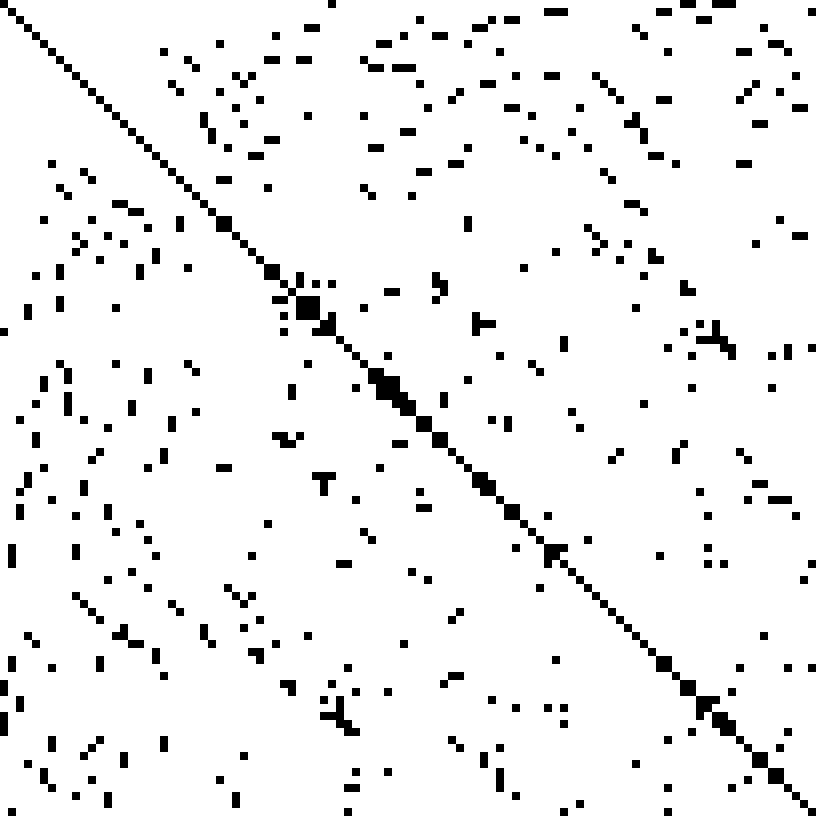
\includegraphics[width=0.35\textwidth]{assets/figures/Finite_element_sparse_matrix.png}
\centering
\caption{A sparse matrix obtained when solving a finite element problem in two dimensions. The non-zero elements are shown in black \cite{SparseMatrixPNG}.}
\end{figure}

\paragraph*{}
There is many formats for storing sparse matrices, we will only present one of them here since it's the only one we will use. This format is the \textbf{\acrfull{csr}}. In this format the row indices are compressed and replaced by an array of \textit{offsets}. A \acrshort{csr} matrix is represented by the following parameters:
\begin{itemize}
    \item The number of rows in the matrix.
    \item The number of columns in the matrix.
    \item The number of \textbf{\acrfull{nnz}} in the matrix.
    \item The row offsets vector of length \texttt{number of rows + 1} that represents the starting position of each row in the columns and values vector.
    \item The column indices vector of length \texttt{\acrshort{nnz}} that contains the column indices of the corresponding elements in the values vector.
    \item The values vector of length \texttt{\acrshort{nnz}} that holds all nonzero values of the matrix.
\end{itemize}

\begin{figure}[h]
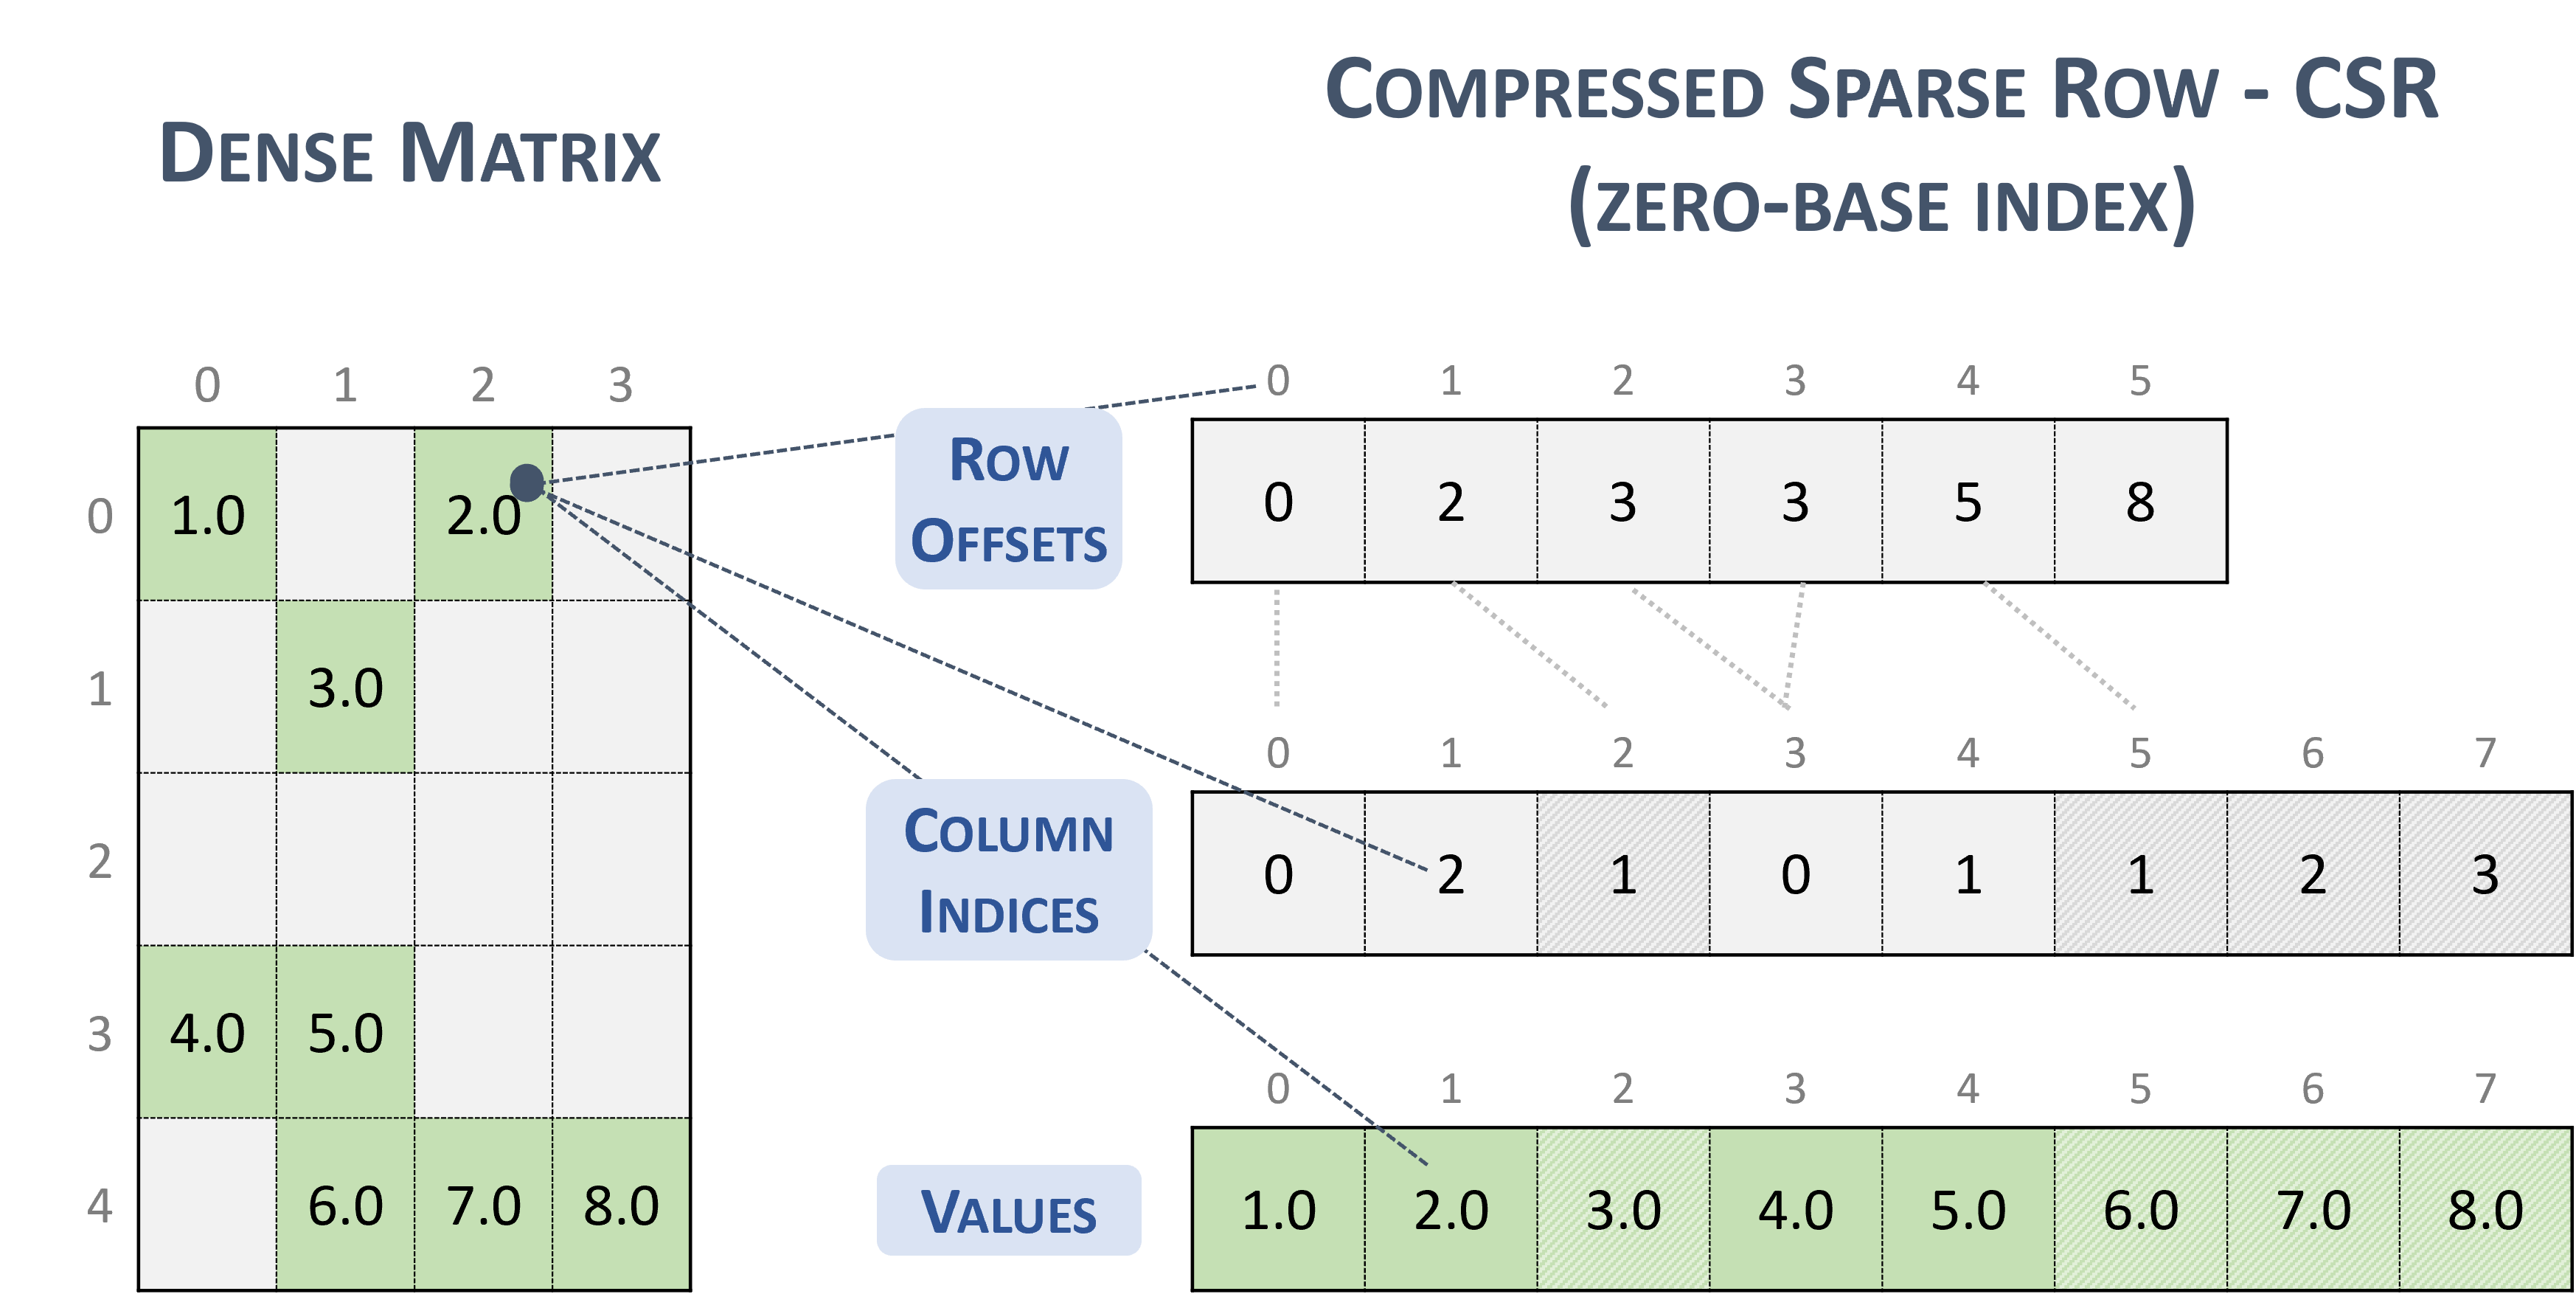
\includegraphics[width=0.6\textwidth]{assets/figures/csr.png}
\centering
\caption{CSR matrix format \cite{cuSPARSE}.}
\end{figure}


\section{Numerical Methods}
\paragraph*{}
Numerical analysis is the study of algorithms that use numerical approximation (as opposed to symbolic manipulations) for the problems of mathematical analysis. It is the study of numerical methods that attempt to find approximate solutions of problems rather than the exact ones.

\subsection{Finite Precision Arithmetic}
\paragraph*{}
Numerical computing is based on the well-known floating-point representation of numbers,
of the form
\begin{align*}
    x=smb^e
\end{align*}
where $s$ is the sign of $x$, $m$ its mantissa, $b$ the basis (usually $b$=2) and $e$ the exponent. Therefore, during computations, numbers are in general subject to \textit{roundoff error}.
The widely-used IEEE 754 \cite{ieee-754} norm for representing floating point numbers and computing with them ensures that
\begin{align*}
    \text{for all } x \in \mathbb{R}, \text{there exists } \varepsilon, \lvert \varepsilon \rvert < \varepsilon_{\text{mach}} \text{  such that } \text{fl}(x) = x(1+\varepsilon)
\end{align*}
where $x \mapsto \text{fl}(x)$ is the operator converting a number to its floating point representation and $\varepsilon_{\text{mach}}$, ofter called "machine epsilon" or "machine precision", is the maximum modulus of relative round-off error.

\paragraph*{}
Throughout this work, we essential focus on two floating point precision,
\begin{itemize}
    \item 32-bit floating point (\texttt{float} in \CC), whose $\varepsilon_{\text{mach}} = 1.19\text{e-}07$
    \item 64-bit floating point (\texttt{double} in \CC), whose $\varepsilon_{\text{mach}} = 2.22\text{e-}16$
\end{itemize}


\subsection{BLAS and LAPACK}
\paragraph*{}
\textbf{\acrfull{blas}} \cite{blas} is a specification that prescribes a set of low-level routines for performing common linear algebra operations such as vector addition, scalar multiplication, dot products, linear combinations, and matrix multiplication.

\paragraph*{}
\acrshort{blas} functionality is categorized into three sets of routines called "levels", which correspond to both the chronological order of definition and publication, as well as the degree of the polynomial in the complexities of algorithms. Level 1 \acrshort{blas} operations typically take linear time, $O(n)$, Level 2 operations quadratic time $O(n^2)$ and Level 3 operations cubic time $O(n^3)$.

\paragraph*{}
\textbf{\acrfull{lapack}} \cite{lapack} is a standard software library for numerical linear algebra. It provides routines for solving systems of linear equations and linear least squares, eigenvalue problems, and singular value decomposition.

\paragraph*{}
When we program numerical linear algebra algorithms, we rely on these libraries to maximize the performances of the computations, since their implementations are often optimized for speed on a particular machine, so using them can bring substantial performance benefits. This is especially true when these operations are performed on a \acrshort{gpu}. GPUs scale much better than CPUs as the size of the data increases \cite{CPUvsGPU2019}. Therefore, we typically prefer implementing algorithms that use matrix-vector or matrix-matrix operations when utilizing a GPU.

\section{Graphical Processing Units}
\paragraph*{}
\acrfull{gpu} is a specialized electronic circuit initially designed to accelerate computer graphics and image processing. Because basic numerical linear algebra operations play crucial roles in real time 3D computer graphics, GPUs are designed for this set of operations. Numerical linear algebra applications can achieve significantly higher performance when using GPUs, as they provide greater peak performance and bandwidth compared to multi-core \acrshort{cpu}s.

\paragraph*{}
The figure below illustrates the main differences in hardware architecture between CPUs and GPUs. The transistor counts associated with various functions are represented abstractly by the relative sizes of the different shaded areas.

\begin{figure}[h]
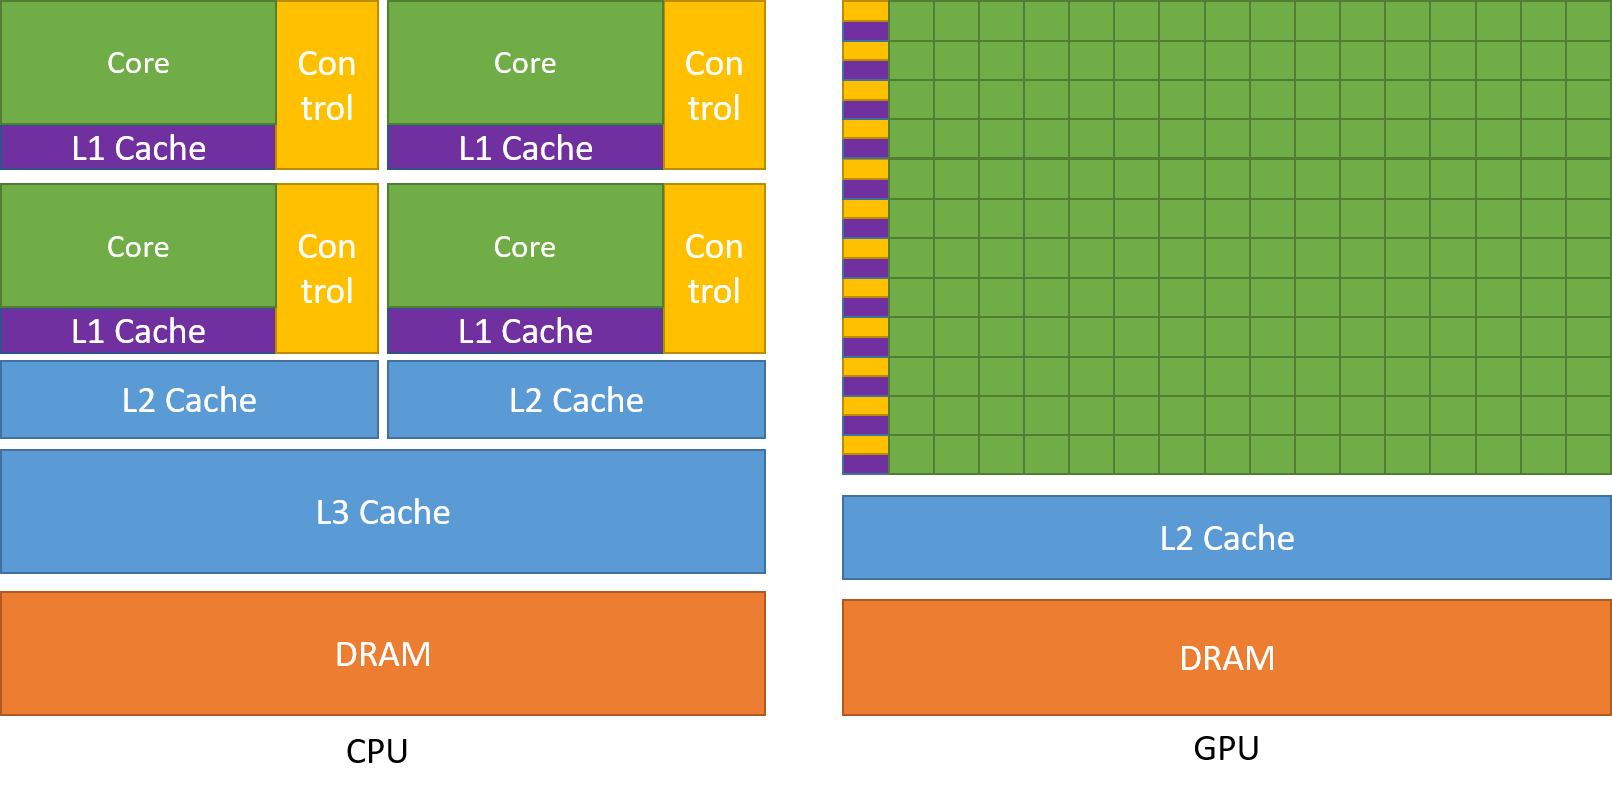
\includegraphics[width=\textwidth]{assets/figures/gpu-devotes-more-transistors-to-data-processing.png}
\centering
\caption{Comparing the relative capabilities of the basic elements of CPU and GPU architectures \cite{cuda}.}
\end{figure}

\paragraph*{}
Concerning the programming model of GPUs, we distinguish the \textit{host} and the \textit{device}. The host refers to the CPU and its memory, while the device refers to the GPU and its memory. Code run on the host can manage memory on both the host and device, and also launches kernels which are functions executed on the device. These kernels are executed by many GPU threads in parallel. However, host cannot access directly memory allocated on the device and vice versa. Therefore, device computing often require additional memory transfers between host and devices.

\newpage
\section{The Eigenvalue Problem}
\subsection{Definition}
\paragraph*{}
The \textbf{(standard) eigenvalue problem} is as follows.
\paragraph*{}
Given a square matrix $A \in \mathbb{R}^{n\times n}$, find $\lambda \in \mathbb{C} \text{ and } \mathbf{x} \in \mathbb{C}^n, \mathbf{x} \neq \mathbf{0}$, such that
\begin{align}\label{eq:1}
    A\mathbf{x}=\lambda\mathbf{x}
\end{align}

or, equivalently, such that 
\begin{align}\label{eq:2}
    (A-\lambda I)\mathbf{x} = \mathbf{0}
\end{align}
Let the pair $(\lambda, \mathbf{x})$ be a solution of \eqref{eq:1} or \eqref{eq:2}. Then 
\begin{itemize}
    \item $\lambda$ is called an \textbf{eigenvalue} of $A$
    \item $\textbf{x}$ is called an \textbf{eigenvector} corresponding to $\lambda$
    \item $(\lambda,\mathbf{x})$ is called \textbf{eigenpair} of $A$
    \item The set $\sigma(A)$  of \textit{all} eigenvalues of $A$ is called \textbf{spectrum} of $A$
\end{itemize}
\paragraph*{}
The \textbf{(generalized) eigenvalue problem} is as follows.

\paragraph*{}
Given two square matrices $A,B \in \mathbb{R}^{n\times n}$, find $\lambda \in \mathbb{C}$ and $\mathbf{x} \in \mathbb{C}, \mathbf{x} \neq \mathbf{0}$, such that
\begin{align}
    A\mathbf{x}=\lambda B \mathbf{x},
\end{align}

or, equivalently, such that 
\begin{align}
    (A-\lambda B)\mathbf{x} = \mathbf{0}
\end{align}

\subsection{Application}\label{chapt:application}
\paragraph*{}
In structural engineering, modal analysis uses the overall mass and stiffness of a structure to find the various periods at which it will naturally resonate. This process helps identify the natural frequencies (resonant frequencies) and corresponding mode shapes, which are critical in understanding how the structure will respond to dynamic loads such as wind, earthquakes, or mechanical vibrations.

\paragraph*{}
The undamped free vibration of structures result in a generalized linear eigenvalue problem
\begin{align}
    M \ddot{\mathbf{u}} + K \mathbf{u} = 0
\end{align}
where the $K$ and $M$ matrices are the stiffness and mass matrices, respectively, $\mathbf{u}$ is the displacement vector, and $\ddot{\mathbf{u}}$ is the acceleration. The solutions of these problems are of the form
\begin{align}
    \mathbf{u} = \boldsymbol{\phi} \cos(\omega t)
\end{align}

Introducing $\lambda = \omega^2$, differentiating twice, and reordering results in the form of the typical generalized linear eigenvalue problem
\begin{align}
    (K-\lambda M)\boldsymbol{\phi} = 0
\end{align}

Since the frequency range of interest in these problems is the lower end of the spectrum, it advisable to use the spectral transformation with $\sigma$ a chosen \textit{shift},
\begin{align} \label{eq:shift}
    \mu = \frac{1}{\lambda - \sigma}
\end{align}
This will change the problem into 
\begin{align}\label{eq:9}
    (K - \sigma M)\boldsymbol{\phi}=\frac{1}{\mu}M\boldsymbol\phi
\end{align}
The eigenvectors are invariant under the spectral transformation, and the eigenvalues may be recovered as
\begin{align}
    \lambda = \frac{1}{\mu} + \sigma
\end{align}

\section{Krylov subspace methods}
\paragraph*{}
Krylov subspace methods \cite{Krylov1931} have been ranked as the 3rd with the greatest influence on the development and practice of science and engineering in the 20th century \cite{Dongarra2000}. Indeed it have become a very useful and popular tool for solving large sets of linear and nonlinear equations, and large eigenvalue problems. One of the reason for their popularity is their simplicity and their generality. These methods have been increasingly accepted as efficient and reliable alternative to the more expensive methods that are usually employed for solving dense problems. This trend is likely to accelerate as models are becoming more complex and give rise to larger and larger matrix problems.

\paragraph*{}
The $n$-th \textbf{Krylov subspace} generated by $A\in \mathbb{R}^{n\times n}$ and $\mathbf{b} \in \mathbb{R}^n$ is the linear subspace spanned by the images of $\mathbf{b}$ under the first $n$ powers of $A$, that is,
\begin{align}
    \mathcal{K}_n(A,\mathbf{b}) = \text{span}\{\mathbf{b}, A\mathbf{b},A^2\mathbf{b},...,A^{n-1}\mathbf{b}\}
\end{align}


\section{Arnoldi Algorithm}\label{seq:arnoldi}
\paragraph*{}
The \textbf{Arnoldi iteration} \cite{Arnoldi1951} is an iterative eigenvalue algorithm. Arnoldi finds and approximation to the eigenvalues and eigenvectors of general matrices by constructing an orthonormal basis of the Krylov subspace, which makes it particularly useful when dealing with large sparse matrices.  

\paragraph*{}
An intuitive method for finding the largest eigenvalue of a given $m\times m$ matrix $A$ is the power iteration \cite{Mises1929}: starting with an arbitraty initial vector $\mathbf{b}$, calculate $A\mathbf{b}, A^2\mathbf{b}$,... normalizing the result after every application of the matrix $A$.

\paragraph*{}
This sequence converges to the eigenvector corresponding to the eigenvalue with the largest absolute value $\boldsymbol{\lambda_1}$. However, much potentially useful computations is wasted by only using the final result, $A^{n-1}\mathbf{b}$. This suggests that instead, we store the intermediate results and form the so-called \textit{Krylov matrix}:
\begin{align}
    \mathcal{K}_n = [\mathbf{b}, A\mathbf{b},A^2\mathbf{b}, ..., A^{n-1}\mathbf{b}]
\end{align}
The columns of this matrix are not in general orthogonal, but we can extract an orthogonal basis, via a method such as Gram-Schmidt algorithm. The resulting set of vectors is thus an orthogonal basis of the Krylov subspace $\mathcal{K}_n(A,\mathbf{b})$. We may expect the vectors of this basis to span good approximations of the eigenvectors corresponding to the $n$ largest eigenvalues.

\begin{algorithm}
\caption{Arnoldi Algorithm}\label{alg:arnoldi}
\begin{algorithmic}[1]
\Require $A \in \mathbb{C}^{n\times n},\text{ an arbitrary vector } \mathbf{b} \in \mathbb{C}^n$
\Ensure $ \mathcal{Q}_k=[\mathbf{q}_1,...,\mathbf{q}_k] \text{ and } \mathcal{H}_k \in \mathbb{C}^{(k+1)\times k}$
\State $\mathbf{q_1} = \mathbf{b}/\lVert \mathbf{b} \rVert_2$
\For{$j=1,...,k-1$}
    \State $\mathbf{w} = A\mathbf{q_j}$ 
    \For{$i=1,...,j$}\LineComment{Gram-Schmidt orthogonalization}
        \State $h_{ij}=\mathbf{q}_i^*\mathbf{w}$
        \State $\mathbf{w} = \mathbf{w}-h_{ij} \mathbf{q}_i$
    \EndFor
    \State $h_{j+1,j} = \lVert \mathbf{w} \rVert$
    \State $\mathbf{q}_{j+1} = \mathbf{w}/h_{j+1,j}$
\EndFor
\end{algorithmic}
\end{algorithm}

\paragraph*{}
Let $\mathcal{Q}_k$ the unitary matrix whose columns $\mathbf{q}_1,...,\mathbf{q}_k$ are the orthonormal basis for $\mathcal{K}_k(A,\mathbf{b})$ generated by the Arnoldi algorithm, and let $\mathcal{H}_k$ be the $(k+1)\times k$ upper Hessenberg matrix defined at the $k$-th stage of the algorithm. We remove that last row of the matrix $\mathcal{H}_k$ , then these matrices satisfy
\begin{align}\label{eq:arnoldi}
    \mathcal{H}_k = \mathcal{Q}_k^*A\mathcal{Q}_k
\end{align}
If  $k<n$, then $\mathcal{H}_k$ is a low-rank approximation to $A$ and the eigenvalues of $\mathcal{H}_k$ may be used as approximations for the eigenvalues of $A$. The eigenvalues of $\mathcal{H}_k$ are called \textit{Ritz eigenvalues}. Since $\mathcal{H}_n$ is a Hessenberg matrix of modest size, its eigenvalues can be computed efficiently, for instance with the QR algorithm \cite{Francis1961}.


\section{Lanczos Algorithm}
\paragraph*{}
The Lanczos algorithm \cite{Lanczos1950}, is the Arnoldi algorithm specialized to the case where $A$ is symmetric. However, we obtain some significant computational savings in this special case. Since $\mathcal{H}_k$ is both symmetric and Hessenberg, it is tridiagonal. This means that in the inner loop of the Arnoldi algorithm \refalg{alg:arnoldi},  the range $1 \text{ to } j$ can be replaced by $j-1 \text{ to } j$. Thus instead of the $j+1$-terms recurrence at step $j$, the Lanczos iteration involves just a $3$-term recurrence. The result is that each step of the Lanczos iteration is much cheaper than the corresponding step of the Arnoldi iteration.

\paragraph*{}
Let us write $\alpha_j=h_{j,j}$ and $\beta_j=h_{j+1,j} \text{ for } j=1,...,k$. Then $\mathcal{H}_k$ becomes
\begin{align*}
    \mathcal{T}_k = 
    \begin{bmatrix}
    \alpha_1    & \beta_1   &           &               &                \\
    \beta_1     & \alpha_2  & \beta_2   &               &                \\
                & \beta_2   & \alpha_3  & \ddots        &                \\
                &           & \ddots    & \ddots        & \beta_{k-1}   \\
                &           &           & \beta_{k-1}   & \alpha_{k}
  \end{bmatrix}
\end{align*} 

\begin{algorithm}
\caption{Lanczos Algorithm}\label{alg:lanczos}
\begin{algorithmic}[1]
\Require $A \text{ a } n\times n \text{ symmetric matrix, an arbitrary vector } \mathbf{b}$ of size $n$
\Ensure $ \mathcal{Q}_k=[\mathbf{q}_1,...,\mathbf{q}_k] \text{ and } \mathcal{T}_k$ the $k\times k$ tridiagonal matrix
\State $\mathbf{q_0} = \mathbf{0}, \quad \beta_0 = 0$
\State $\mathbf{q}_1 = \mathbf{b}/\lVert \mathbf{b} \rVert_2 \quad Q_1 = [\mathbf{q}_1]$
\For{$j=1,2,...,k-1$}
    \State $\mathbf{w} = A\mathbf{q}_j$
    \State $\alpha_j = \mathbf{q}_j^T \mathbf{w}$
    \State $\mathbf{w} = \mathbf{w} - \beta_{j-1}\mathbf{q}_{j-1}-\alpha_j\mathbf{q}_j$ 
    \State $\beta_j = \lVert \mathbf{w} \rVert_2$
    \State $\mathbf{q}_{j+1} = \mathbf{w}/\beta_j   \quad \mathcal{Q}_{j+1}=[\mathcal{Q}_j \ \mathbf{q}_{j+1}]$
\EndFor
\end{algorithmic}
\end{algorithm}

\paragraph*{}
Some modifications, re-arrangements or additional steps may be applied to this algorithm for reasons of numerical stability in a finite arithmetic context. We won't detail them here but it can be find in the literature such as in \cite{Golub1996}.

\paragraph*{}
In context of large sparse matrices, \textit{block} methods can offers advantages over classical methods. By performing operations on blocks of vectors instead of on single vector, we can take advantage of \acrshort{blas} 3 routines instead of \acrshort{blas} 2, and therefore speed-up the computation time. For iterative eigensolvers, block methods reduce the number of iterations required to resolve a cluster of nearby eigenvalues. For some applications, block methods are necessary for computing all the desired eigenvalues to the desired accuracy; they are not (just) a performance optimization.

\paragraph*{}
The block Lanczos algorithm is similar to the classical Lanczos algorithm, the Krylov subspace is formed by the column vectors of the $n\times ks$ matrix $\mathcal{Q}_k=[Q_1,...,Q_k]$, where $s$ is the block size.
Here is a block version of the Lanczos algorithm. \cite{Grimes1994}.

\begin{algorithm}
\caption{Block Lanczos Algorithm}\label{alg:block_lanczos}
\begin{algorithmic}[1]
\Require $H \text{ a } n\times n $ symmetric matrix, an arbitrary matrix $Q_1$ such as $Q_1^*Q_1 = I_s$
\Ensure $ \mathcal{Q}_k=[Q_1,...,Q_k] \text{ and } \mathcal{T}_k$ the $ks\times ks$ block tridiagonal matrix
\State $Q_0 = \mathbf{0}, \quad B_0 = \mathbf{0}$
\For{$j=1,2,...,k-1$}
    \State $W = HQ_j$
    \State $A_j = Q_j^T W$
    \State $W = W - Q_{j-1}B_{j-1}^T - Q_j A_j$
    \State $Q_{j+1}, B_{j} = \mathtt{QR}(W)$ \LineComment{$Q_{j+1}$ is orthogonal and $B_{j}$ is upper triangular}
\EndFor
\end{algorithmic}
\end{algorithm}

\paragraph*{}
The matrices $Q_j$ and $W$ for $j=1,2,..k$ are $n \times s$, whereas $A_j$ and $B_j$ are $p\times p$, with $A_j$ symmetric. The algorithm also defines a $ks\times ks$ block tridiagonal matrix $\mathcal{T}_k$

\begin{align*}
    \mathcal{T}_k = 
    \begin{bmatrix}
    A_1 & B_1   &       &           &           \\
    B_1 & A_2   & B_2   &           &           \\
        & B_2   & A_3   & \ddots    &           \\
        &       & \ddots& \ddots    & B_{k-1}   \\
        &       &       & B_{k-1}   & A_{k}
  \end{bmatrix}
\end{align*}

\paragraph*{}
The \texttt{QR} subroutines used in the algorithm compute the QR factorization of the matrix $W$. This operation factorize a $m \times n$ matrix $A$ into a product $A=QR$ of a orthogonal $m \times m$ matrix $Q$ and a upper triangular $n\times n$ matrix $R$. There are several methods for actually computing the QR decomposition, such as the Gram–Schmidt process, Householder transformations\cite{Householder1958}, or Givens rotations. Each has a number of advantages and disadvantages.

\paragraph*{}
The next step is to consider the generalized symmetric eigenproblem \eqref{eq:9}. We finally obtain the Shifted Block Lanczos algorithm \cite{Grimes1994}.

\begin{algorithm}
\caption{Shifted Block Lanczos Algorithm}\label{alg:shifted_block_lanczos}
\begin{algorithmic}[1]
\Require $H \text{ a } n\times n $ symmetric matrix, an arbitrary matrix $Q_1$ such as $Q_1^TMQ_1 = I_s$
\Ensure $ \mathcal{Q}_k=[Q_1,...,Q_k] \text{ and } T_k$ the $ks\times ks$ block tridiagonal matrix
\State $Q_0 = \mathbf{0}, \quad B_0 = \mathbf{0}$
\For{$j=1,2,...,k-1$}
    \State $W = (K-\sigma M)^{-1}(MQ_j)$
    \State $A_j = W^T (M Q_j)$
    \State $W = W - Q_{j-1}B_{j-1}^T - Q_j A_j$
    \State $Q_{j+1}, B_{j} = \text{\texttt{M-QR}}(W)$ \LineComment{$Q_{j+1}$ is M-orthogonal and $B_{j}$ is upper triangular}
\EndFor
\end{algorithmic}
\end{algorithm}

The \texttt{M-QR} routine computes also the $QR$ factorization of the matrix $W$ as explained for the previous algorithm \refalg{alg:block_lanczos} but instead of computing $Q$ an orthogonal matrix, it computes $Q$ as a M-orthogonal matrix (i.e. $Q^TMQ=I)$.

\paragraph*{}
This algorithm can capture the eigenvalues around the given shift $\sigma$. Sometimes, the algorithm struggle to find all the eigenvalues close to the given shift after a lot of iterations. One strategy is to restart the algorithm with a different shift $\sigma$, to capture additional nearby eigenvalues.




\newpage
\section{Quadratic Eigenvalue Problem}
\subsection{Definition}
\paragraph*{}
The \textbf{\acrfull{qep}} is as follows.
\paragraph*{}
Given $M,C, K \in \mathbb{C}^{n\times n}$, find $\lambda \in \mathbb{C}$, left and right nonzero eigenvectors $\mathbf{x}, \mathbf{y} \in \mathbb{C}^n$, such that
\begin{align}
    (\lambda^2 M + \lambda C + K)\mathbf{x} = 0, \quad \mathbf{y}^*(\lambda^2M + \lambda C + K) = 0
\end{align}

\subsection{Application}
\paragraph*{}
In the section \ref{chapt:application}, we described the application on the case of modal analysis and undamped free vibration of structures. The consideration of damping makes the analysis closer to the reality. The damping effect is represented by the presence of the damping matrix.

\paragraph*{}
The quadratic eigenvalue problems result from the differential equation
\begin{align}
    M \ddot{\mathbf{u}} + C \dot{\mathbf{u}} + K\mathbf{u} = 0
\end{align}
where $C$ is the damping matrix, $\dot{\mathbf{u}}$ refers to the velocity. The solution of this homogeneous system is of the form 
\begin{align}
    \mathbf{u} = e^{\lambda t}\boldsymbol{\sigma}
\end{align}\label{eq:qep}
where $\boldsymbol{\sigma}$ is a complex vector and the $\lambda$ eigenvalue is also complex in general. Substitution of the last equation and its time derivatives gives the characteristic equation
\begin{align}
    ( \lambda^2 M + \lambda C + K)\boldsymbol{\Phi} = 0
\end{align}

The \acrshort{qep} has a wide range of applications beyond structural analysis. Tisseur and Meerbergen \cite{Tisseur2001} provide a excellent survey on the \acrshort{qep} and its various applications.  

\paragraph*{}
Two approaches are well-known to solve quadratic eigenvalue problems and quadratic system of equations. One approach finds an appropriate linearization that results in linear eigenvalue problems or a linear system of equations. Another approach projects larger sparse quadratic problem onto a lower dimensional subspace, and subsequently produce a small, dense QEP or a system of equations. The first approach has a drawback that it increases the condition number due to linearization that double the size of the problem. 

\paragraph*{}\label{seq:quad_eig}
The second approach can be summarize in the following steps:
\begin{enumerate}
    \item Set $A=-K^{-1}C$ and $B=-K^{-1}M$ and use an algorithm to construct a lower dimensional subspace matrix $\mathcal{Q}$.
    \item Compute reduced order coefficient matrices $M_m = \mathcal{Q}^T M \mathcal{Q}$, $C_m = \mathcal{Q}^T C \mathcal{Q}$ and $K_m =  \mathcal{Q}^T K \mathcal{Q}$.
    \item Use dense QEP solver to solve $(\theta^2M_m + \theta C_m + K_m)\mathbf{g} = 0$ for Ritz paris $(\theta_i, \mathbf{g}_i)$.
    \item Transform Ritz vectors $\mathbf{g}_i$ into full-order vectors $\boldsymbol{\Phi}_i=\mathcal{Q}\mathbf{g}_i$ and normalize it.
\end{enumerate}
Note that we never explicitly compute the $A$ and $B$ matrices by inverting $K$. Usually, we only need the result of the matrix-vector product $\mathbf{x} = A\mathbf{r}$. We can implicitly calculate the result $\mathbf{x}$ by solving the linear system
\begin{align}
    \mathbf{x} & = A\mathbf{r} \\
    \mathbf{x} & = -K^{-1}C \mathbf{r} \\
    K \mathbf{x} & = -C \mathbf{r} \label{eq:implicit_mv}
\end{align}
Which in the end only implies two matrix-vector products and a linear solve.

\paragraph*{}
We will use the state-of-the-art algorithm \textbf{\acrfull{toar}} \cite{toar2016} for solving such QEPs by constructing reduced order problem.






\newpage
\chapter{Work Done}
\paragraph*{}
In general, there are two main approaches to accelerating an application using a GPU. The first approach involves rewriting the application so that all computations are performed on the GPU. The second approach is a hybrid method that offloads specific operations to the GPU, targeting those that are likely to be faster on the GPU. Both methods have their own advantages and disadvantages.

\paragraph*{}
The advantage of the first approach is that it fully exploits the GPU's potential, with no latency from memory transfers between the host and the device. On the other hand, the hybrid method can be more easily integrated into existing code and allows for focusing on highly parallelizable operations. However, this approach involves additional memory transfers, which might cause overhead.

\paragraph*{}
In our case, we chose the hybrid approach which is obviously the easier to start with. We identified 3 main computational costs in the Shifted Block Lanczos algorithm \refalg{alg:shifted_block_lanczos}.
\begin{itemize}
    \item The matrix-vector products (line 3)
    \item The resolution of linear systems (line 3)
    \item The orthogonalization procedures (line 5)
\end{itemize}

\paragraph*{}
We decided to address first the orthogonalization procedure, because the matrix-vector product acceleration was already in progress, and the resolution of linear systems was harder to begin with.

\section{Orthogonalization Procedures}\label{seq:ortho}
\paragraph*{}
The goal of this work is to experiment with various orthogonalization procedures and explore whether they can be accelerated using the GPU. This involves considering two key aspects: performance and numerical stability. Our primary focus is on performance, but we must also ensure a minimum level of stability.

\paragraph*{}
An orthogonalization procedure is a procedure that, given a set of vectors $S=[\mathbf{v}_n,...,\mathbf{v}_n]$, generate an orthogonal set $S'=[\mathbf{u}_1,...,\mathbf{u}_n]$ that spans the same n-dimensional subspace.

\paragraph*{}
We will try different algorithms and measured their performances as well as their numerical stability in order to find the best one for our use case. Here is a table of all the acronyms of the studied algorithms.

\begin{table}[h!]
\centering
\begin{tabular}{|l|l|} 
 \hline
 CGS & Classical Gram-Schmidt \\ 
 MGS & Modified Gram-Schmidt \\
 CGS2 & Classical Gram-Schmidt with reorthogonalization \\
 BCGS & Block Classical Gram-Schmidt \\
 BMGS & Block Modified Gram-Schmidt \\
 BCGS2 & Block Classical Gram-Schmidt with reorthogonalization \\
 CholQR & Cholesky QR \\
 \hline
\end{tabular}
\caption{Acronyms for orthogonalization algorithm}
\label{table:1}
\end{table}

\subsection{Gram-Schmidt Algorithm and its Variants}
\paragraph*{}
Gram-Schmidt Algorithm is a well known way of finding a set of two or more vectors that are perpendicular to each other.

\begin{algorithm}
\caption{\texttt{CGS}}\label{alg:cgs}
\begin{algorithmic}[1]
\Require $X = [\mathbf{x}_1,...,\mathbf{x}_n] \in \mathbb{R}^{m\times n}$
\Ensure $ Q=[\mathbf{q}_1,...,\mathbf{q}_n] \in \mathbb{R}^{m\times n}, R \in \mathbb{R}^{n\times n}$ such that $QR = X$ and $Q^TQ=I_n$
\For{$i=1,...,n$}
    \State $\mathbf{r}_i = \mathbf{x}_i$
    \For{$j=1,...,i-1$}
        \State $\mathbf{r}_i = \mathbf{r}_i - (\mathbf{q}_j^T\textcolor{red}{\mathbf{x}_i})\mathbf{q}_j$
    \EndFor
    \State $\mathbf{q}_i = \mathbf{r}_i/ \lVert \mathbf{r}_i \rVert_2$
\EndFor
\end{algorithmic}
\end{algorithm}

\paragraph*{}
We can rewrite this algorithm in matrix notation to take advantages of the speed-up of matrix-vector product over vector-vector dot product. This allows us to leverage \acrshort{blas} 2 operations. This version is even more interesting on GPU because it leverages matrix-vector product parallelism.  

\begin{algorithm}
\caption{\texttt{CGS} (matrix notation)}\label{alg:cgs_mat}
\begin{algorithmic}[1]
\Require $X = [\mathbf{x}_1,...,\mathbf{x}_n] \in \mathbb{R}^{m\times n}$
\Ensure $ Q=[\mathbf{q}_1,...,\mathbf{q}_n] \in \mathbb{R}^{m\times n}, R \in \mathbb{R}^{n\times n}$ such that $QR = X$ and $Q^TQ=I_n$
\State $Q = X$
\For{$i=1,...,n$}
    \State $R_{1:i-1,i} = Q_{:,1:i-1}^T X_{:,k}$
    \State $Q_{:,k} = X_{:,k} - Q_{:,1:k-1} R_{1:k-1,k}$
    \State $R_{k,k} = \lVert Q_{:,k} \rVert$
    \State $Q_{:,k} = Q_{:,k}/R_{k,k}$
\EndFor
\end{algorithmic}
\end{algorithm}

\paragraph*{}
It turns out that the Gram-Schmidt procedure we introduced previously suffers from numerical instability: Round-off errors can accumulate and destroy orthogonality of the resulting vectors \cite{cgs1974}. We introduce the modified Gram-Schmidt procedure to help remedy this issue. 

\begin{algorithm}
\caption{\texttt{MGS}}\label{alg:mgs}
\begin{algorithmic}[1]
\Require $X = [\mathbf{x}_1,...,\mathbf{x}_n] \in \mathbb{R}^{m\times n}$
\Ensure $ Q=[\mathbf{q}_1,...,\mathbf{q}_n] \in \mathbb{R}^{m\times n}, R \in \mathbb{R}^{n\times n}$ such that $QR = X$ and $Q^TQ=I_n$
\For{$i=1,...,n$}
    \State $\mathbf{r}_i = \mathbf{x}_i$
    \For{$j=1,...,i-1$}
        \State $\mathbf{r}_i = \mathbf{r}_i - (\mathbf{q}_j^T\textcolor{red}{\mathbf{r}_i})\mathbf{q}_j$
    \EndFor
    \State $\mathbf{q}_i = \mathbf{r}_i/ \lVert \mathbf{r}_i \rVert_2$
\EndFor
\end{algorithmic}
\end{algorithm}

\paragraph*{}
In classical Gram-Schmidt (CGS) we compute the projections of the \textbf{original} $k$-th column vector $\mathbf{x}_k$ onto all left orthogonal column vectors already computed $\{\mathbf{q}_{j}\}_{j=1}^{k-1}$. Then subtract those projections from $\mathbf{x}_k$ :
\begin{align}
    \mathbf{r}_k = (I - Q_{k-1} Q_{k-1}^T)\mathbf{x}_k
\end{align}
In modified Gram–Schmidt (MGS) we compute the projection of the \textbf{computed} $k$-th column vector $\mathbf{x}_k$ onto $\mathbf{q}_1$ and then subtract this projection from $\mathbf{x}_k$. Then do the same sequentially for all $\{\mathbf{q}_{j}\}_{j=1}^{k-1}$ :
\begin{align}
    \mathbf{r}_k = (I - \mathbf{q}_k\mathbf{q}_k^T)...(I - \mathbf{q}_1\mathbf{q}_1^T)\mathbf{x}_k
\end{align}
See the difference highlighted in red in \refalg{alg:cgs} and \refalg{alg:mgs}.

\paragraph*{}
There is an even more numerically stable version of the Gram-Schmidt algorithm which is the classical Gram-Schmidt algorithm with reorthogonalization (CGS2). By repeating the process of orthogonalization twice, we ensure that orthogonality of the set of vectors only depends on the machine precision. This is also known as the Kahan-Parlett "twice-is-enough" algorithm \cite{Parlett1998}.

\begin{algorithm}
\caption{\texttt{CGS2}}\label{alg:cgs2}
\begin{algorithmic}[1]
\Require $X \in \mathbb{R}^{m\times n}$
\Ensure $ Q \in \mathbb{R}^{m\times n}, R \in \mathbb{R}^{n\times n}$ such that $QR = X$ and $Q^TQ=I_n$
\State $Q = X$
\For{$i=1,...,n$}
    \State $R^{(1)} = Q_{:,1:i-1}^T X_{:,k}$ \LineComment{1st CGS step}
    \State $Q^{(1)} = X_{:,k} - Q_{:,1:k-1} R^{(1)}$
    \State $R^{(2)} = Q_{:,1:i-1}^T Q^{(1)}$ \LineComment{2nd CGS step}
    \State $Q_{:,k} = Q^{(1)} - Q_{:,1:k-1} R^{(2)}$
    \State $R_{k,k} = \lVert Q_{:,k} \rVert$
    \State $Q_{:,k} = Q_{:,k}/R_{k,k}$
    \State $R_{1:i-1,i} = R^{(1)} + R^{(2)}$
\EndFor
\end{algorithmic}
\end{algorithm}

\subsection{Cholesky QR Factorization}
\paragraph*{}
The Cholesky QR factorization, or \texttt{CholQR} is also another algorithm that could be interesting because it doesn't require to work column by column sequentially (which is a bottleneck for GPU acceleration). This algorithm only rely on 3 kernels calls, that are all part of the \acrshort{lapack} library :
\begin{itemize}
    \item \texttt{SYRK}, compute $A = X^TX$ which makes $A$ matrix \acrshort{spd}
    \item \texttt{CHOL}, compute $R$ with Cholesky factorization $RR^T=\mathtt{Chol}(A)$
    \item \texttt{TRSM}, compute $Q = AR^{-1}$ by solving the triangular matrix equation $XR=A$
\end{itemize}
However, this algorithm is not suited for all sizes of matrices because the $X^TX$ operation squares the condition number of the matrix $A$.

\begin{algorithm}
\caption{\texttt{CholQR}}\label{alg:cholqr}
\begin{algorithmic}[1]
\Require $X \in \mathbb{R}^{m\times n}$
\Ensure $ Q\in \mathbb{R}^{m\times n}, R \in \mathbb{R}^{n\times n}$ such that $QR = X$ and $Q^TQ=I_n$
\State $A = X^TX$
\State $R = \mathtt{Chol(A)}$ \LineComment{Cholesky factorization}
\State $Q = AR^{-1}$
\end{algorithmic}
\end{algorithm}




\subsection{Block Gram-Schmidt Variants}
\paragraph*{}
As the orthogonalization procedures we are studying are part of a block version of the Lanczos algorithm \refalg{alg:shifted_block_lanczos}, we also investigate block version of the standard Gram-Schmidt algorithm introduced in the previous section. For the same reason, we only consider algorithms that work left-to-right i.e., only information from the $k$ first blocks of $Q$ and $X$ is necessary for generating $Q_{k+1}$.

\paragraph*{}
This work is essentially based on the work of Carson et al.\cite{Carson2022} which provides a great comprehensive categorization of block Gram-Schmidt algorithms (BGS), particularly those used in Krylov subspace methods to build orthonormal bases one block of vectors at a time.

\paragraph*{}
In the following, we consider a matrix $X \in \mathbb{R}^{m\times n}, m\gg n$ which is partitioned into a set of $p$ \textit{block vectors}, each of size $m\times s$, i.e.
\begin{align*}
    X = [X_1,X_2,...,X_p]
\end{align*}
We also consider the QR factorization $X=QR$, where $Q=[Q_1,...,Q_p] \in \mathbb{R}^{m \times n}$ has the same structure than $X$ and $R\in \mathbb{R}^{n \times n}$.
(To remember the meaning of subscript, note that $m > n > p > s$ which is in the alphabetical order and $n=ps$).

\paragraph*{}
We can decompose a BGS in two main part, the \textit{intra}-block orthogonalization and the \textit{inter}-block orthogonalization. We need to orthogonalize every block to each others (\texttt{InterOrtho}) and every vector within a block to each other (\texttt{IntraOrtho}). The \textit{inter}-block orthogonalization algorithm is independent of the \textit{intra}-block orthogonalization algorithm, which means we can mix any \texttt{InterOrtho} with any \texttt{IntraOrtho}.

\begin{figure}[h]
    \centering
    \includesvg{assets/figures/block_ortho.svg}
    \caption{Block Orthogonalization Diagram}
    \label{fig:block_orthogo}
\end{figure}

\paragraph*{}
The \texttt{IntraOrtho} routines have been presented in the previous section. We will now describe the \texttt{InterOrtho} ones independently. For simpler notation, we denote $A_{1:k}$ the sub matrix $A' = [A_1,...,A_k]$.

\begin{algorithm}
\caption{\texttt{BCGS}}\label{alg:bcgs}
\begin{algorithmic}[1]
\Require $X \in \mathbb{R}^{m\times n}$
\Ensure $ Q\in \mathbb{R}^{m\times n}, R \in \mathbb{R}^{n\times n}$ such that $QR = X$ and $Q^TQ=I_n$

\State $Q_1, R_{1,1} = \mathtt{IntraOrtho}(X_1)$
\For{$i=1,...,p-1$}
    \State $R_{1:i,i+1} = Q_{1:i}^T X_{i+1}$
    \State $W = X_{i+1} - Q_{1:i} R_{1:i,i+1}$
    \State $Q_{i+1}, R_{i+1,i+1} = \mathtt{IntraOrtho}(W)$
\EndFor
\end{algorithmic}
\end{algorithm}

\begin{algorithm}
\caption{\texttt{BMGS}}\label{alg:bmgs}
\begin{algorithmic}[1]
\Require $X \in \mathbb{R}^{m\times n}$
\Ensure $ Q\in \mathbb{R}^{m\times n}, R \in \mathbb{R}^{n\times n}$ such that $QR = X$ and $Q^TQ=I_n$

\State $Q_1, R_{1,1} = \mathtt{IntraOrtho}(X_1)$
\For{$i=1,...,p-1$}
    \State $W = X_{i+1}$
    \For{$j=1,...,i-1$}
        \State $R_{j,i+1} = Q_{j}^T W$
        \State $W = W - Q_j R_{j,i+1}$
    \EndFor
    \State $Q_{i+1}, R_{i+1,i+1} = \mathtt{IntraOrtho}(W)$
\EndFor
\end{algorithmic}
\end{algorithm}


\begin{algorithm}
\caption{\texttt{BCGS2}}\label{alg:bcgs2}
\begin{algorithmic}[1]
\Require $X \in \mathbb{R}^{m\times n}$
\Ensure $ Q\in \mathbb{R}^{m\times n}, R \in \mathbb{R}^{n\times n}$ such that $QR = X$ and $Q^TQ=I_n$

\State $Q_1, R_{1,1} = \mathtt{IntraOrtho}(X_1)$
\For{$i=1,...,p-1$}
    \State $R_{1:i;i+1}^{(1)} = Q_{1:i}^T X_{i+1}$ \LineComment{1st BCGS step}
    \State $W = X_{i+1} - Q_{1:i} R_{1:i,i+1}^{(1)}$
    \State $Q^{(1)}, R_{i+1,i+1}^{(1)} = \mathtt{IntraOrtho}(W)$
    \State $R_{1:i,i+1}^{(2)} = Q_{1:i}^T Q^{(1)}$ \LineComment{2nd BCGS step}
    \State $W = Q^{(1)} - Q_{1:i} R_{1:i,i+1}^{(2)}$
    \State $Q_{i+1}, R_{i+1,i+1}^{(2)} = \mathtt{IntraOrtho}(W)$
    \State $R_{1:i,i+1} = R_{1:i,i+1}^{(1)} + R_{1:i,i+1}^{(2)} R_{i+1,i+1}^{(1)}$
    \State $R_{i+1,i+1} = R_{i+1,i+1}^{(2)} R_{i+1,i+1}^{(1)}$
\EndFor
\end{algorithmic}
\end{algorithm}

\newpage
\subsection{Numerical Properties}
\paragraph*{}
All of this orthogonalization procedures have different numerical properties. Since we use these algorithms to orthogonalize matrices, we are interested in a upper bounds on the loss of orthogonality due to round off errors during computations. 
Let $\hat{Q}$ be the result of an orthogonalization of $X$. We measure the loss of orthogonality as the quantity 
\begin{align}\label{eq:ortho_loss}
    \lVert I_n - \hat{Q}^T \hat{Q} \rVert
\end{align}
for some norm $\lVert \cdot \rVert$. We take the Euclidean norm, unless otherwise noted. We express the upper bound of \eqref{eq:ortho_loss} in terms of the machine precision $O(\varepsilon)$ and the matrix condition number $\kappa(X)$ which is the ratio between its largest and smallest singular value.

\paragraph*{}
The following table summarize the upper bound on the loss of orthogonality after intra-block orthogonalization.

\begin{figure}[h]
\begin{center}
\begin{tabular}{ |c|c|c|c| } 
 \hline
 Algorithm & $\lVert I_n - \hat{Q}^T \hat{Q} \rVert$ & Assumption on $\kappa(X)$ & References \\ 
 \hline
 \texttt{CGS} & $O(\varepsilon)\kappa^{n-1}(X)$ & $O(\varepsilon)\kappa(X)<1$ & \cite{cgs1974} \\ 
 \texttt{CholQR} & $O(\varepsilon)\kappa^2(X)$ & $O(\varepsilon)\kappa^2(X)<1$ & \cite{cholQR2015} \\ 
 \texttt{MGS} & $O(\varepsilon)\kappa(X)$ & $O(\varepsilon)\kappa(X)<1$ & \cite{Bjrck1967} \\
 \texttt{CGS2} & $O(\varepsilon)$ & $O(\varepsilon)\kappa(X)<1$ & \cite{Giraud2005},\cite{Abdelmalek1971},\cite{Barlow2013} \\
 \hline
\end{tabular}
\end{center}
\caption{Upper bound on loss of orthogonality for standard orthogonalization algorithms.}
\label{tab:gs_bound}
\end{figure}

\paragraph*{}
We notice that \texttt{CGS} is really unstable, its therefore a bad choice for most of the applications. \texttt{CGS2} doesn't depend on the matrix condition number, which is really interesting even though the computational cost is almost twice of the other ones.

\paragraph*{}
Concerning the BGS, the bound on loss of orthogonality is depending on the bound of the \texttt{IntraOrtho} used. The following table summarize this bounding.

\begin{figure}[h]
\begin{center}
\begin{tabular}{ |c|c|c|c|c| } 
 \hline
 Algorithm & \texttt{IntraOrtho} bound & $\lVert I_n - \hat{Q}^T \hat{Q} \rVert$ & Assumption on $\kappa(X)$ & References \\ 
 \hline
 \texttt{BCGS} & $O(\varepsilon)$ & $O(\varepsilon)\kappa^{n-1}(X)$ & $O(\varepsilon)\kappa(X)<1$ & conjectured in \cite{Carson2022} \\ 
 \texttt{BMGS} & $O(\varepsilon) \kappa(X)$ &$O(\varepsilon)\kappa^2(X)$ & $O(\varepsilon)\kappa(X)<1$ &  \cite{Jalby1991} \cite{Carson2022} \\
 \texttt{BMGS} & $O(\varepsilon)$ &$O(\varepsilon)\kappa(X)$ & $O(\varepsilon)\kappa(X)<1$ & \cite{Jalby1991} \cite{Carson2022} \\
 \texttt{BCGS2} & $O(\varepsilon)$ &$O(\varepsilon)$ & $O(\varepsilon)\kappa(X)<1$ & \cite{Barlow2013}  \\
 \hline
\end{tabular}
\end{center}
\caption{Upper bound on loss of orthogonality for block orthogonalization algorithms.}
\label{tab:bgs_bound}
\end{figure}

\paragraph*{}
Knowing those theoretical bounding, we will try to reproduce these results and explore the behaviour of \texttt{InterOrtho} with different \texttt{IntraOrtho}. We denote this composition with the symbol $\circ$. For example, \texttt{BCGS} $\circ$ \texttt{CGS} is the Block Classical Gram-Schmidt algorithm that uses classical Gram-Schmidt algorithm as \texttt{IntraOrtho} routine.


\newpage
\subsection{Numerical Benchmarks}
\paragraph*{}
The goal is to measure the loss of orthogonality against the condition number of the matrix. We will carry out our experiments exclusively in double precision, using \texttt{float64} in other words. Therefore the machine precision is $\varepsilon = 1\text{e-}16$. This is because in real-life use cases, the orthogonality is too sensible and critical to use single precision.

\paragraph*{}
To generate matrices with a specific condition number $\kappa(X)$, we generate a $m \times n$ matrix
\begin{align*}
    X = U\Sigma V^T
\end{align*}
where $U, V \in \mathbb{R}^{m \times n}$ are orthogonal matrices and $\Sigma \in \mathbb{R}^{n \times n}$ is a diagonal matrices whose entries are such that 
\begin{align*}
\kappa(X) = \frac{\sigma_{max}(\Sigma)}{\sigma_{min}(\Sigma)}
\end{align*}
For this we use the  \texttt{LATMS} routine from \acrshort{lapack}.

\begin{figure}[h]
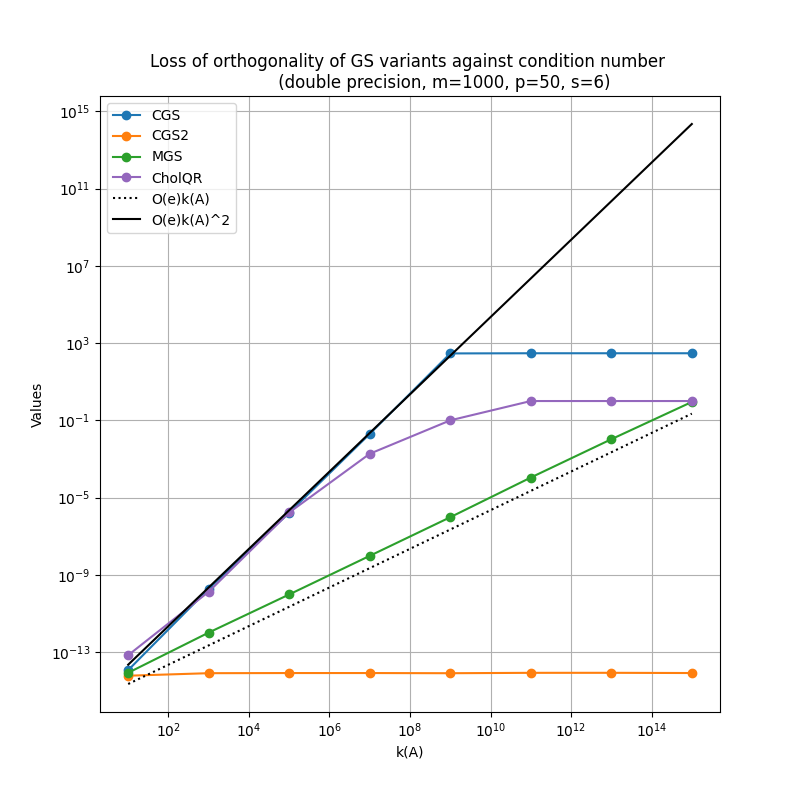
\includegraphics[width=0.67\textwidth]{results/orthogo_bench/numerical_bench_gs.png}
\centering
\caption{Loss of orthogonality measurement of GS variants}
\label{fig:num_gs}
\end{figure}

\paragraph*{}
The figure \ref{fig:num_gs} shows us the result of the measurements. We can see that they are consistent with the theoretical results in \ref{tab:gs_bound}. \cgsi is very interesting because the loss of orthogonality doesn't depend on the condition number of the matrix, which makes it a better solution for badly conditioned matrices. In general, \mgs is sufficient for common matrices. 

\paragraph*{}
The \texttt{CholQR} algorithm could have been a good alternative to Gram-Schmidt even if it's bounded by the square of the condition number. This is because we are not using big block sizes in the Lanczos algorithm, therefore we could expect a low condition number for each block. Nevertheless, after some preliminaries results on \texttt{CholQR} performances, we decided to not continue with this algorithm as it was much slower than Gram-Schmidt algorithms on GPU. For an orthogonalization of a block of 6 vectors of size 1e6, the \texttt{CholQR} was 100 times slower. This algorithm might be interesting on bigger block sizes though, but in our case, we were contrainted to small block sizes.


\begin{figure}[h!]
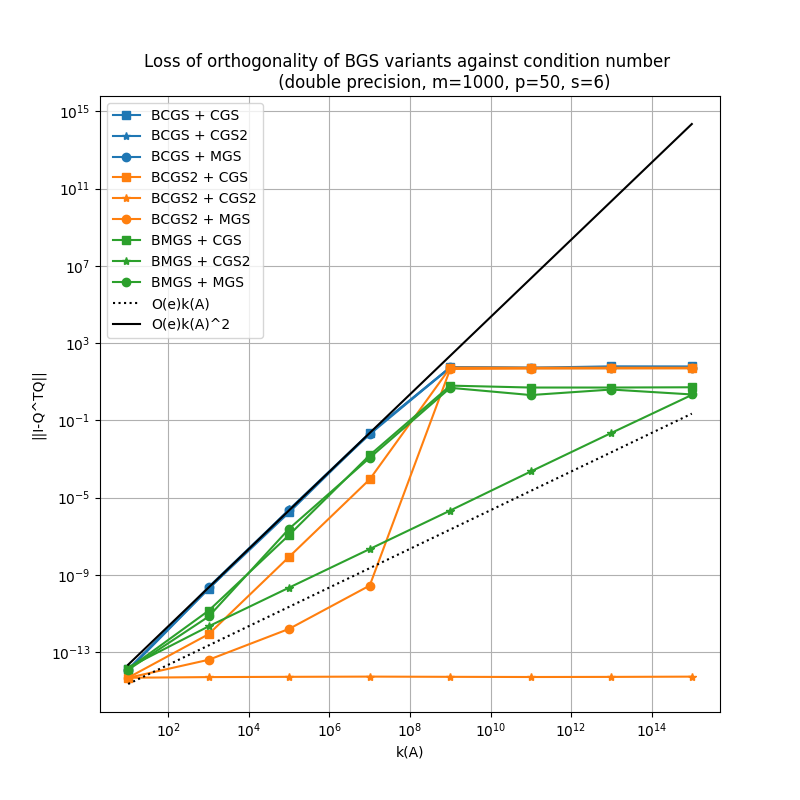
\includegraphics[width=0.67\textwidth]{results/orthogo_bench/numerical_bench_bgs.png}
\centering
\caption{Loss of orthogonality measurement of BGS variants}
\label{fig:num_bgs}
\end{figure}

\paragraph*{}
The figure \ref{fig:num_bgs} is also consistent with the theoretical bounds given in \ref{tab:bgs_bound}. We learn that the choice of the \texttt{IntraOrtho} can make a big difference depending on the \texttt{InterOrtho}. First, \texttt{BCGS} is so unstable, no matter what \texttt{IntraOrtho} is used, that we won't consider it as an option for a real use case. Thus, we can consider only \texttt{MGS} $\circ$ \texttt{CG2}, \texttt{BCGS2} $\circ$ \texttt{MGS} or \texttt{BCGS2} $\circ$ \texttt{CGS2}. The choice between this options will depends on the performances of the algorithms and the type of matrices to deal with.

\paragraph*{}
There are also other Gram-Schmidt variants that use optional reorthogonalization. Those variants are really interesting for a CPU implementation, but since we target a GPU implementation, we won't explore this options for performance reasons.

\newpage
\subsection{Performance Benchmarks}
\paragraph*{}
The aim of this work is to compare the performances of the CPU implementation versus the GPU implementation of the algorithms shown above. For the CPU implementation, we used the \acrfull{mkl} \cite{intelMKL} for the \acrshort{blas} kernels calls. For the GPU implementation, we focused on NVIDIA GPUs since they were the most accessible in the company and the most efficient on the market. So, we used the CUDA programming language as well as the cuBLAS library \cite{cuBLAS} which is the NVIDIA implementation of the \acrshort{blas} standard.

\paragraph*{}
Different metrics are relevant regarding the performance of an algorithm. We decided to measure the \textbf{\acrfull{flops}}, which is the computational power of hardware, such as CPUs or GPUs. It tells us how many floating-point operations the hardware can perform every second. To measure the FLOPS of each algorithm, we divide their flop counts by their execution time. For the GPU implementation, we don't measure the time of data transfers between host and device.

\paragraph*{}
The following table \ref{tab:gs_flops} summarizes the number of flops for basic linear algebra operations \cite{Lapack41} and for GS algorithms. For the GS algorithms, we only give an approximation of the flops count for 
simplicity. For instance, the flops count for \cgs is 
\begin{align*}
    (n-1)\frac{(n-2)}{2} 4m+n(3m+1) = 2mn^2 - 3mn + 4m + n \approx  2mn^2
\end{align*}
Regarding the block GS algorithms, we ignore the number of flops of the \texttt{IntraOrtho} since it is negligible compare to the whole algorithm. For instance in case of \bmgs $\circ$ \texttt{Intra}, the flops count is
\begin{align*}
    flops(\bmgs \circ \mathtt{Intra}) &=  flops(\mathtt{Intra}) + (p-2)\frac{(p-3)}{2}4ms^2 + (p-1)flops(\mathtt{Intra}) \\
    & \approx 2mp^2s^2 + p flops(\mathtt{Intra}) \\
    & \approx 2m p^2 s^2 + pms^2 \\
    & \approx 2mp^2 s^2 \\
    & \approx 2 m n^2, (\text{ since } n=ps)
\end{align*}
As a result, the block version of GS is in the same order of magnitude than the classical ones.

\begin{figure}[h]
\begin{center}
\begin{tabular}{ |c|c|c| } 
    \hline
    Operation & Dimension & Flops \\ 
    \hline
    $\alpha = \mathbf{x}^T \mathbf{y}$ & $\mathbf{x},\mathbf{y} \in \mathbb{R}^n$ & $2n$ \\
    $\mathbf{y} = \mathbf{y} + A\mathbf{x}$ & $A\in \mathbb{R}^{m\times n}, x\in \mathbb{R}^n, y\in \mathbb{R}^m$ & $2mn$ \\
    $C = C + AB$ & $A \in \mathbb{R}^{m\times k}, B \in \mathbb{R}^{k\times n}, C \in \mathbb{R}^{m\times n}$ & $2mnk$ \\
    \hline
    \cgs$(X)$ & $X\in \mathbb{R}^{m\times n}$ & $2mn^2$ \\
    \cgsi$(X)$ & $X\in \mathbb{R}^{m\times n}$ & $4mn^2$ \\
    \mgs$(X)$ & $X\in \mathbb{R}^{m\times n}$ & $2mn^2$ \\
    \bcgs$(X)$ & $X\in \mathbb{R}^{m\times n}$ & $2mn^2$ \\
    \bcgsi$(X)$ & $X\in \mathbb{R}^{m\times n}$ & $4mn^2$ \\
    \bmgs$(X)$ & $X\in \mathbb{R}^{m\times n}$ & $2mn^2$ \\
    
    
    \hline
\end{tabular}
\end{center}
\caption{ Important flop counts }
\label{tab:gs_flops}
\end{figure}


\paragraph*{}
We conducted our benchmarks on two hardware configurations: 
\begin{itemize}
    \item 16 Intel Xeon Gold 6226R and NVIDIA Quadro RTX 4000
    \item 48 Intel(R) Xeon(R) Gold 6342 CPU and Nvidia A100 80GB PCIe
\end{itemize}
The first benchmark was conducted on a regular workstation GPU with not many double precision cores. The processing power is 222.5 GFLOPS in double precision \cite{GpuSpec}. As a result, the GPU implementation is actually slower than the CPU one. Depending on the algorithm, the CPU can be 3 to 6 times faster than the GPU.

\begin{figure}[h]
    \centering
    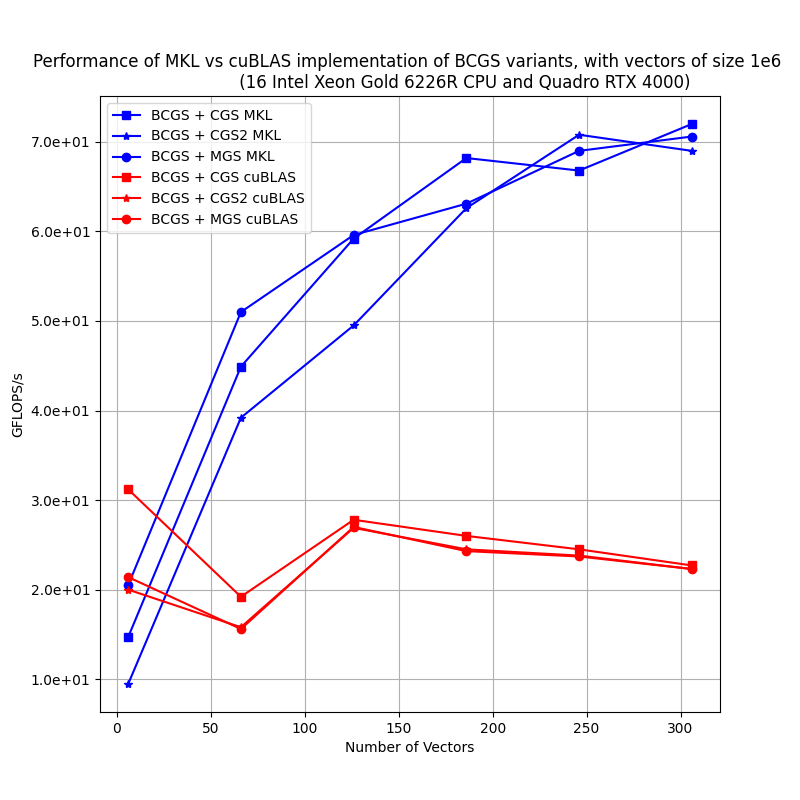
\includegraphics[width=0.49\linewidth]{results/orthogo_bench/flops_bench_bcgs_Quadro4000.png}
    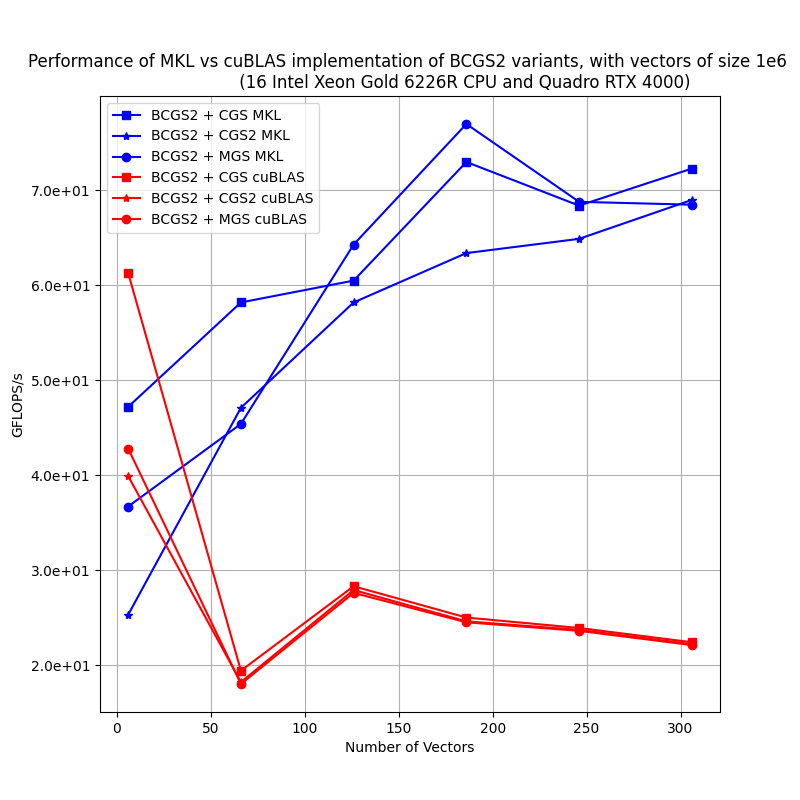
\includegraphics[width=0.49\linewidth]{results/orthogo_bench/flops_bench_bcgs2_Quadro4000.png}
    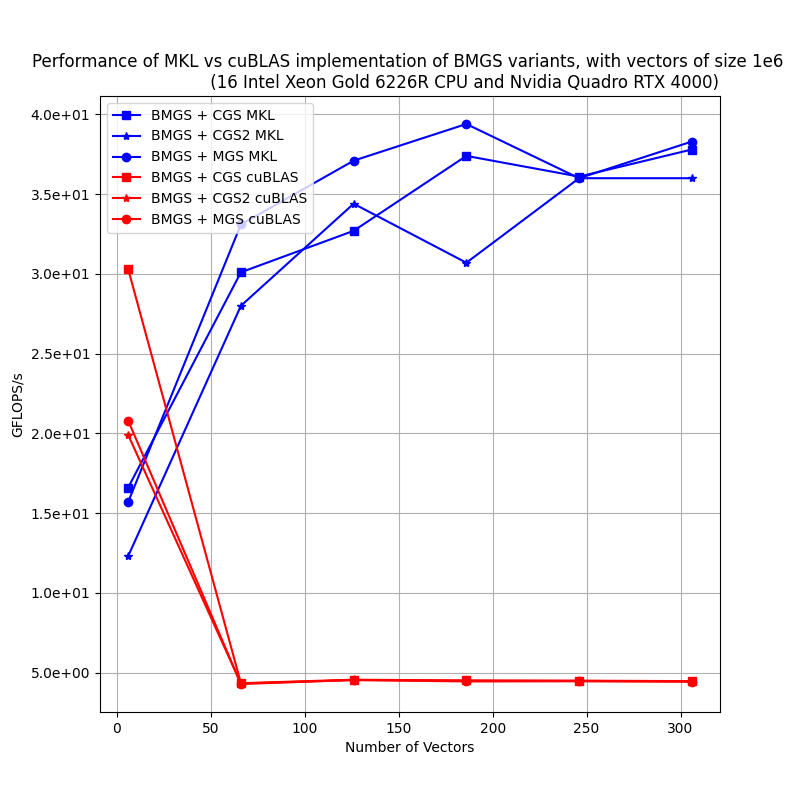
\includegraphics[width=0.49\linewidth]{results/orthogo_bench/flops_bench_bmgs_Quadro4000.png}
    \caption{Benchmark results of CPU vs GPU on NVIDIA Quadro RTX 4000}
    \label{fig:bench_quadro}
\end{figure}

We also conducted the same benchmark on a different GPU to see the difference between a basic workstation GPU and a professional GPU. For this model, the processing power in double precision is 9,700 GFLOPS which makes a huge difference compared to the previous one. This time, the GPU implementation achieved up to 10 times speed-up compared to the CPU as we can see in \ref{fig:bench_A100}.

\begin{figure}[h]
    \centering
    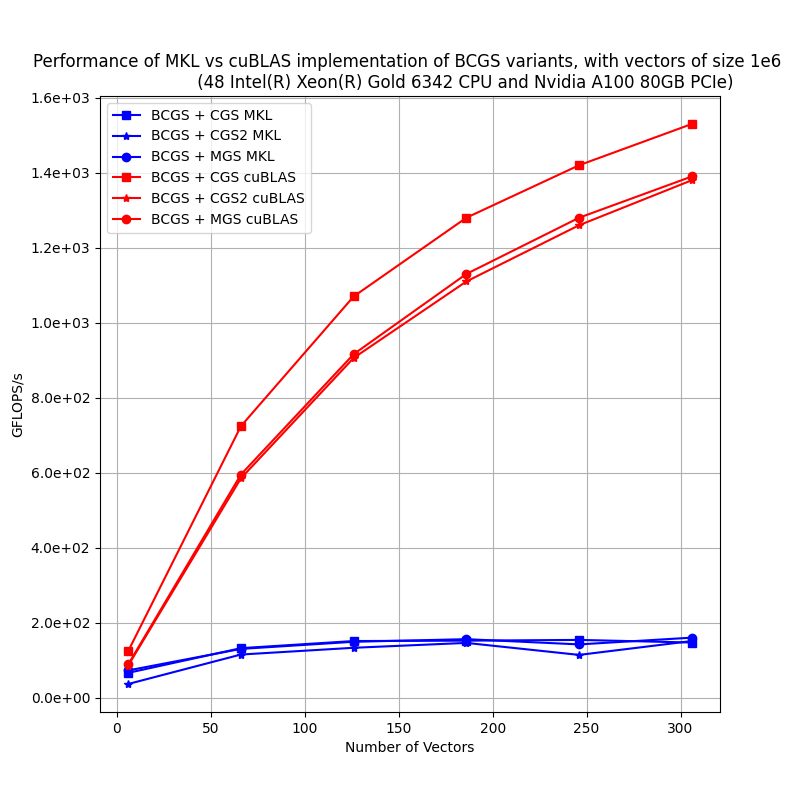
\includegraphics[width=0.49\linewidth]{results/orthogo_bench/flops_bench_bcgs.png}
    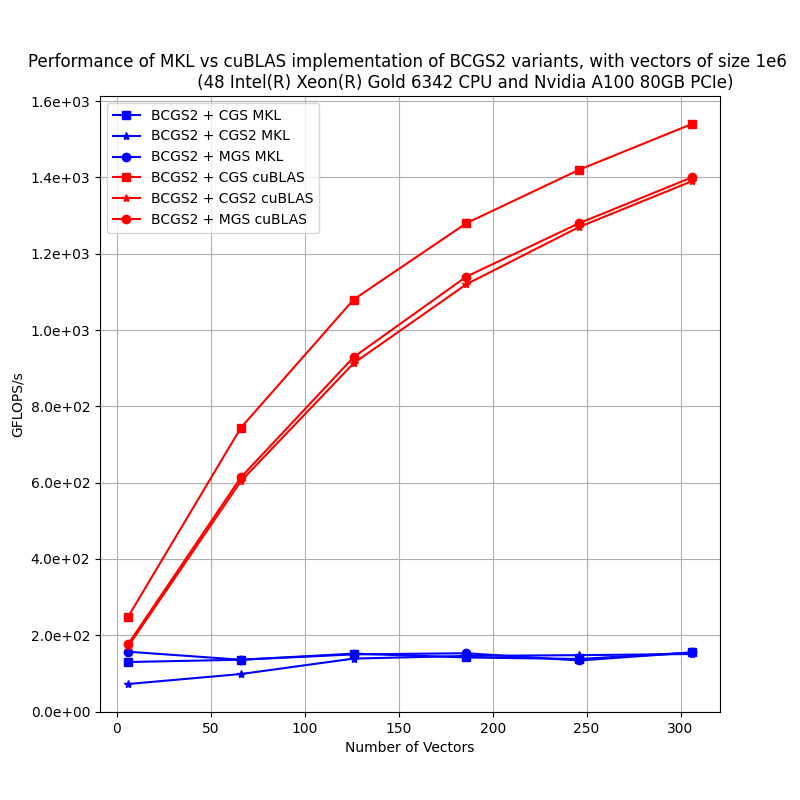
\includegraphics[width=0.49\linewidth]{results/orthogo_bench/flops_bench_bcgs2.png}
    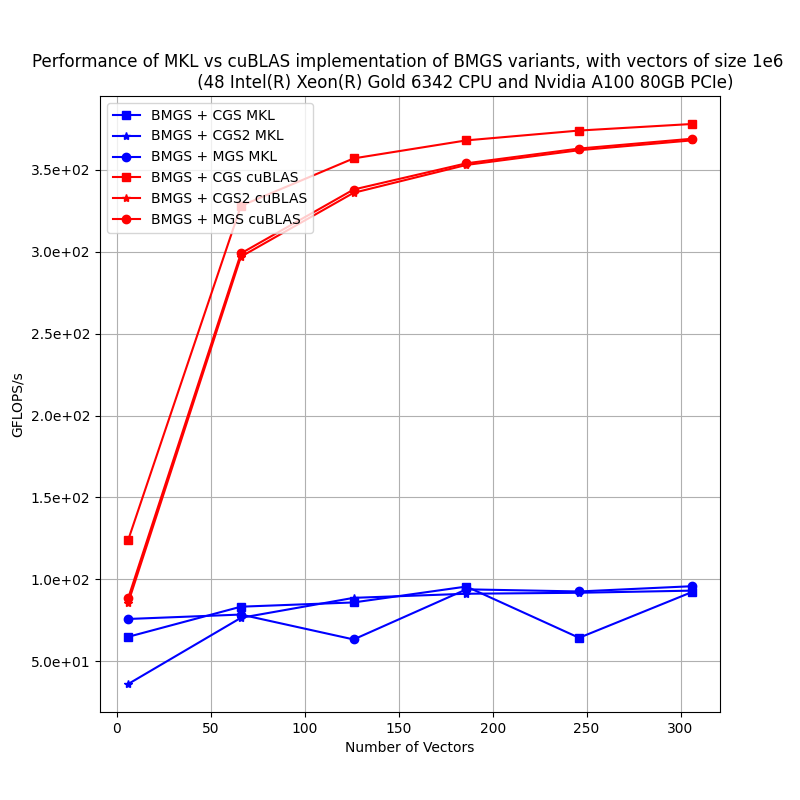
\includegraphics[width=0.49\linewidth]{results/orthogo_bench/flops_bench_bmgs.png}
    \caption{Benchmark results of CPU vs GPU on NVIDIA A100}
    \label{fig:bench_A100}
\end{figure}

\paragraph*{}
Now that we have the results, the question we want to address is which of the tested algorithms is the best fit for our use case. For this, we compare the execution time of each BGS variants as well as their numerical properties. The goal is to find the best trade-off between performance and numerical stability.

\begin{figure}[h]
    \centering
    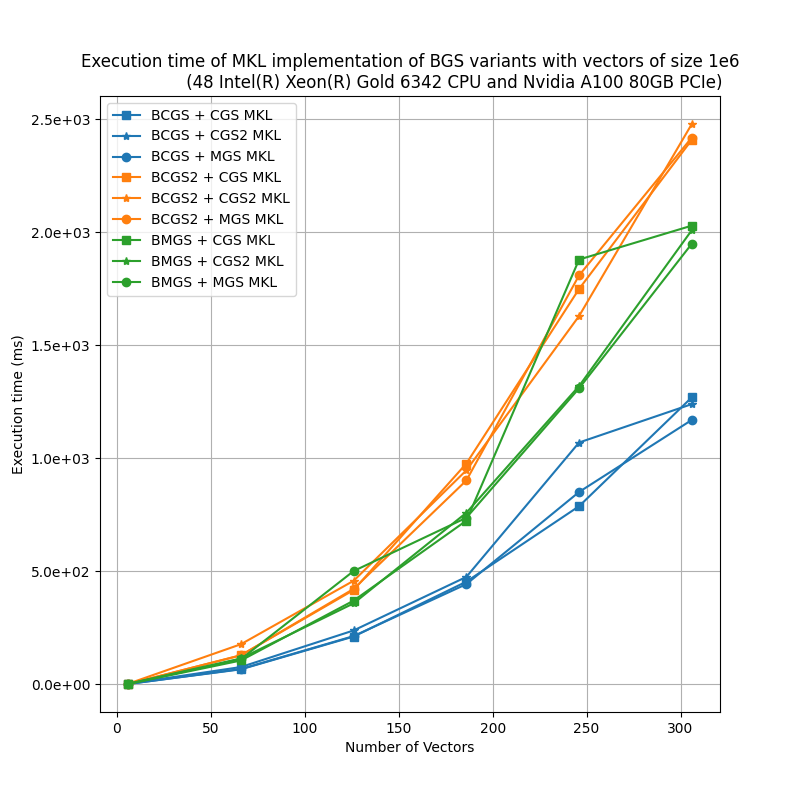
\includegraphics[width=0.49\linewidth]{results/orthogo_bench/time_bench_mkl.png}
    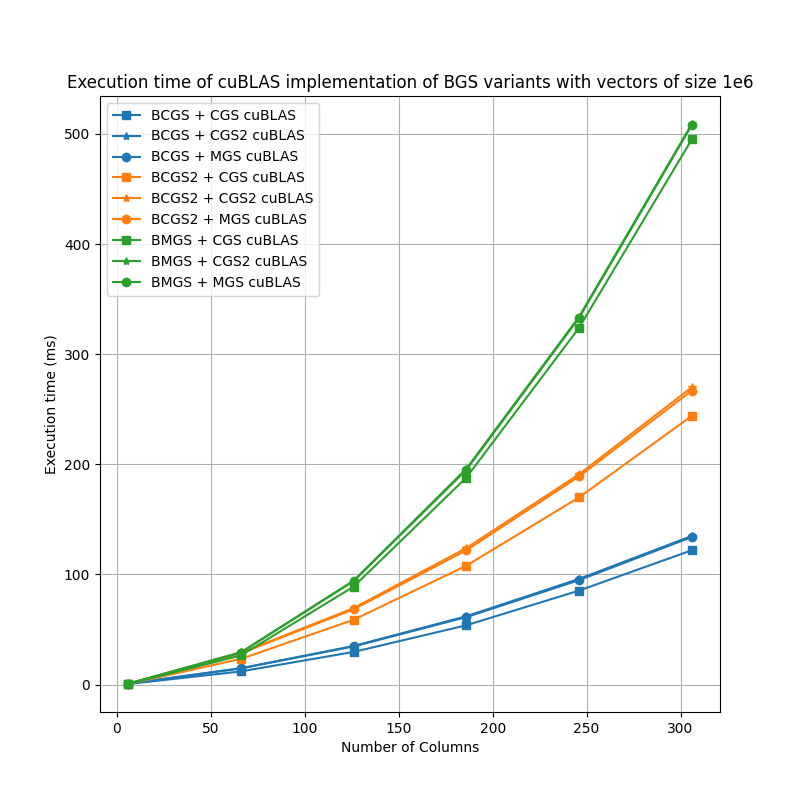
\includegraphics[width=0.49\linewidth]{results/orthogo_bench/time_bench_cublas.png}
    \caption{Execution time benchmark of CPU and GPU}
    \label{fig:bench_A100_time}
\end{figure}

\paragraph*{}
First, we notice that the \texttt{IntraOrtho} subroutines don't have much impact on the performances of the CPU and GPU. This can be explain by the fact that the block size used for these benchmarks was $s=6$ which is a small block size. So the difference between the various GS variants cannot significantly influence the execution time.

\paragraph*{}
Then, regarding the CPU versions, the \bcgs is faster than \bmgs which is faster than \texttt{BCGS2}. The \bcgs being to unstable, we only consider \bmgs and \texttt{BCGS2}. We believe that the \bmgs $\circ$ \cgsi, the \bcgsi $\circ$ \mgs and the \bcgsi $\circ$ \cgsi are each a good solution. The difficulty is to find the right trade-off between numerical stability and performance that fit the use case.

\paragraph*{}
Finally, regarding the GPU versions, the \bcgs is faster than the \bcgsi which is faster than the \texttt{BMGS}. Unlike the CPU version, there is no trade-off to find because the \bcgsi is the fastest and the more stable (not considering \bcgs). Thus, the \bcgsi $\circ$ \cgsi is the best choice on GPU.

\paragraph*{}
To conclude this section, we managed to implement some orthogonalization algorithms that are faster on professional GPU than on CPU and so accelerate algorithms that use orthogonalization. We also demonstrated which one was the better solution regarding the performances and the numerical stability.

\paragraph*{}
Unfortunately, we couldn't integrate the code into the actual Shifted Block Lanczos implementation due to architectural design constraints. Consequently, measuring the GPU acceleration of the entire algorithm was not possible. This will be addressed in future work.







\newpage
\section{Benchmark of a Direct Sparse Solver}\label{seq:cudss}
\paragraph*{}
As said in the previous section, another important computational cost is the solve of a linear system during the Shifted Block Lanczos algorithm. There is many CPU-based direct sparse solvers such as MUMPS \cite{Mumps2001} or PARDISO \cite{Pardiso2000}, but also GPU-accelerated ones such as CHOLMOD \cite{CHOLMOD2008} or GLU \cite{GLU2019}. But NVIDIA released its own direct sparse solver cuDSS \cite{cuDSS}, in November 2023, which was really promising so we decided to test it.

\paragraph*{}
To test this GPU linear solver, we decided to offload the solve of the linear system to the GPU and compare the execution time of this operation with the actual CPU-based direct sparse solver of Ansys. The solve of a linear system such as $A\mathbf{x} = \mathbf{b}$ consist of 3 main phases:
\begin{enumerate}
    \item The \textbf{symbolic factorization} is a preparatory step that focuses on understanding and optimizing the structure of the matrix factors, often involving reordering of the matrix to minimize fill-in and improve computational efficiency during the numerical factorization.
    \item The \textbf{numerical factorization} decompose the matrix into a product of matrices. There are many different matrix factorizations. This step is necessary for the solve of the linear system.
    \item The \textbf{solve} phase which basically solve the linear system using the factorized matrix and the right hand side of the equation.
\end{enumerate}
Sometimes, we need to solve a linear system many times with the same matrix structure, but different numerical factors. In this case, we can perform the symbolic factorization only once, since it only depends on the matrix structure and not the numerical values of the factors. Then, we need to perform the numerical factorization whenever the numerical value of the matrix factors change. Finally, we can perform the solve phase for any right hand side of the linear system.

\paragraph*{}
In the Shifted Block Lanczos algorithm \refalg{alg:shifted_block_lanczos}, the computation involves a matrix-matrix product with the inverse of a matrix, specifically $W = (K-\sigma M)^{-1}(MQ_j)$ (see line 3). However, computing the inverse of $(K-\sigma M)$ is inefficient and sometimes impossible. Since we only require the result of the matrix-matrix product involving $(K-\sigma M)^{-1}$, we can compute it implicitly:
\begin{align}
    W & = (K-\sigma M)^{-1}(MQ_j) \\ 
   (K-\sigma M) W & = (MQ_j)
\end{align}
Thus, we solve, for a given shift $\sigma$, the linear system of equations
\begin{align}
    (K-\sigma M) X = (MQ_j) \label{eq:lanc_solve}
\end{align}

\paragraph*{}
This means that we need to perform symbolic factorization only once for the whole method (even if we restart the algorithm with a different shift $\sigma$). We need also to perform numerical factorization of the matrix $(K-\sigma M)$ for each shift $\sigma$. And finally we need to solve the linear system \eqref{eq:lanc_solve} at each iteration.

\paragraph*{}
We conducted our benchmark on different models and on different hardware configurations. The size of a model is quantified in terms of its \textbf{\acrfull{dof}}. For a given size of a model, the size of the matrices $K$ and $M$ correspond  to the number of \acrshort{dof}. The model size was constrained by the 80GB capacity of the GPU memory. The two hardware configurations were:
\begin{itemize}
    \item \texttt{np} x Intel(R) Xeon(R) Gold 6342 CPU and NVIDIA RTX 6000 Ada Generation
    \item \texttt{np} x Intel(R) Xeon(R) Gold 6342 CPU and NVIDIA H100 PCIe
\end{itemize}
With variable number of cores \texttt{np} from 8 to 32.

\begin{figure}[h!]
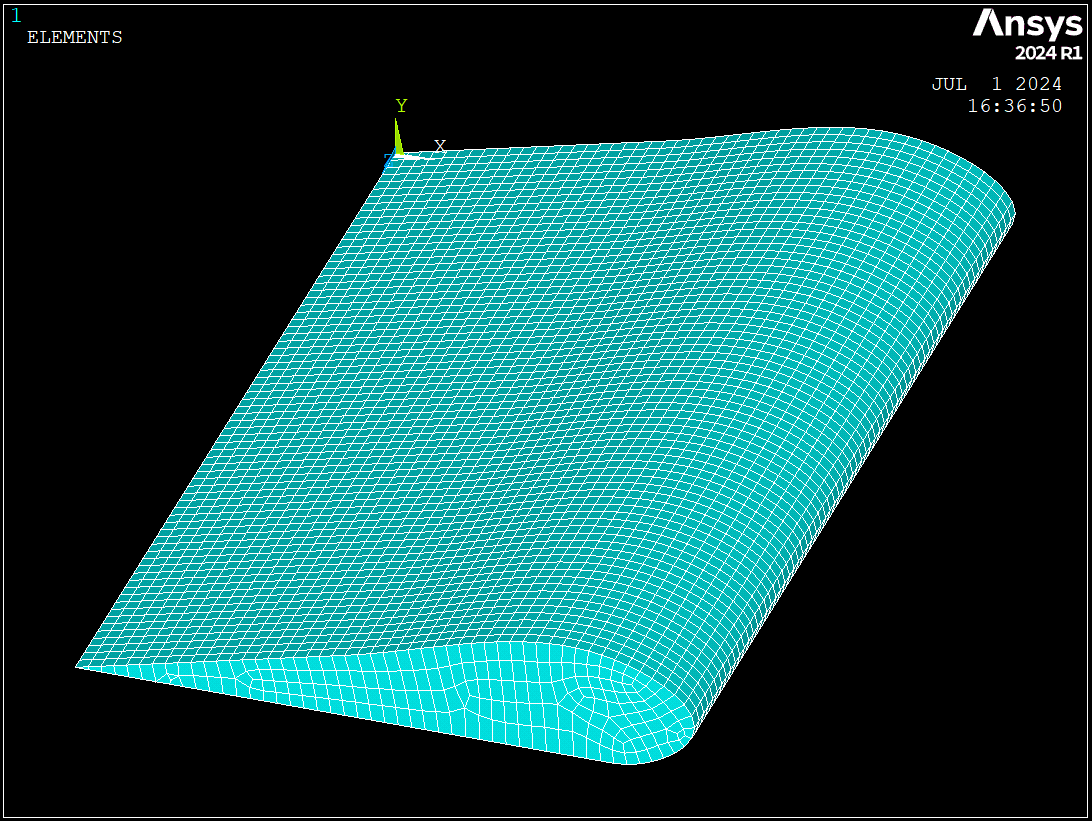
\includegraphics[width=0.65\textwidth]{assets/figures/wing.png}
\centering
\caption{Plane wing model}
\label{fig:wing}
\end{figure}

\begin{figure}[h!]
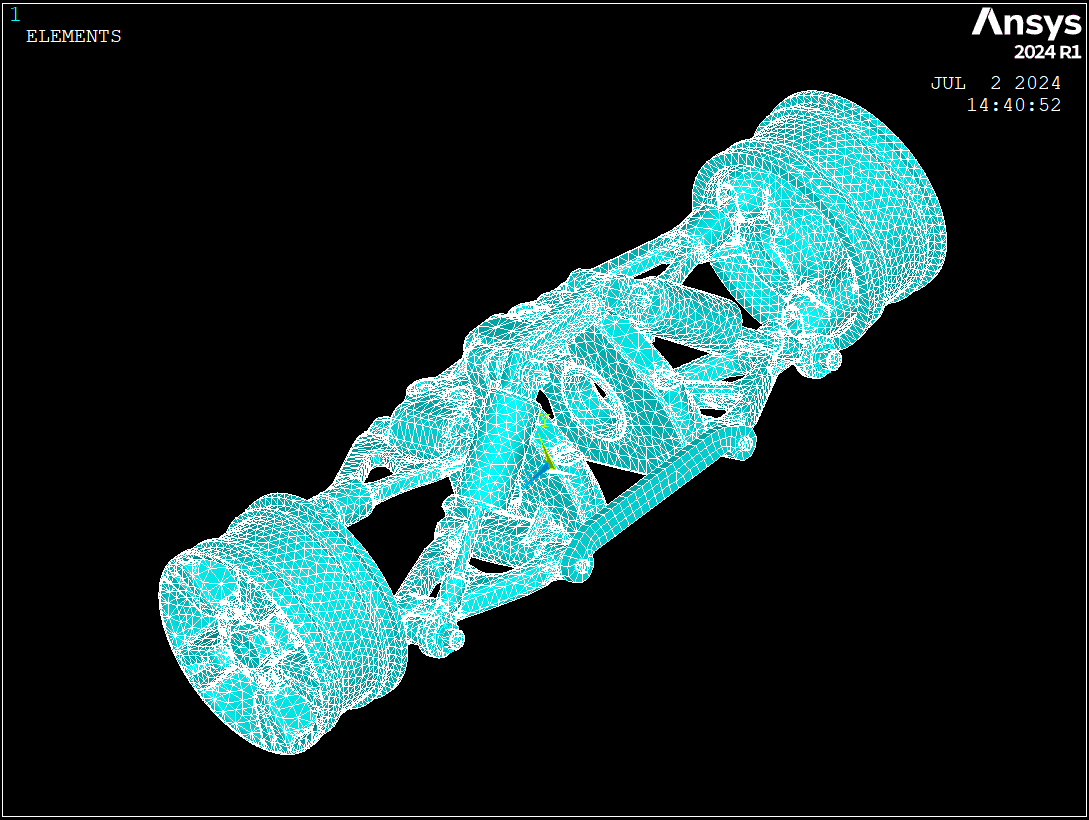
\includegraphics[width=0.65\textwidth]{assets/figures/suspension.png}
\centering
\caption{Suspension model}
\label{fig:suspension}
\end{figure}

\paragraph*{}
We performed modal analysis, searching for 50 eigenfrequencies, on a plane wing model (figure \ref{fig:wing}). This model was available in different sizes.  Our testing covered three versions with 200,000, 1,000,000, and 2,000,000 \acrlong{dof}. We also used a suspension model of 1,000,000 \acrlong{dof} (figure \ref{fig:suspension}).

\begin{figure}[H]
    \centering
    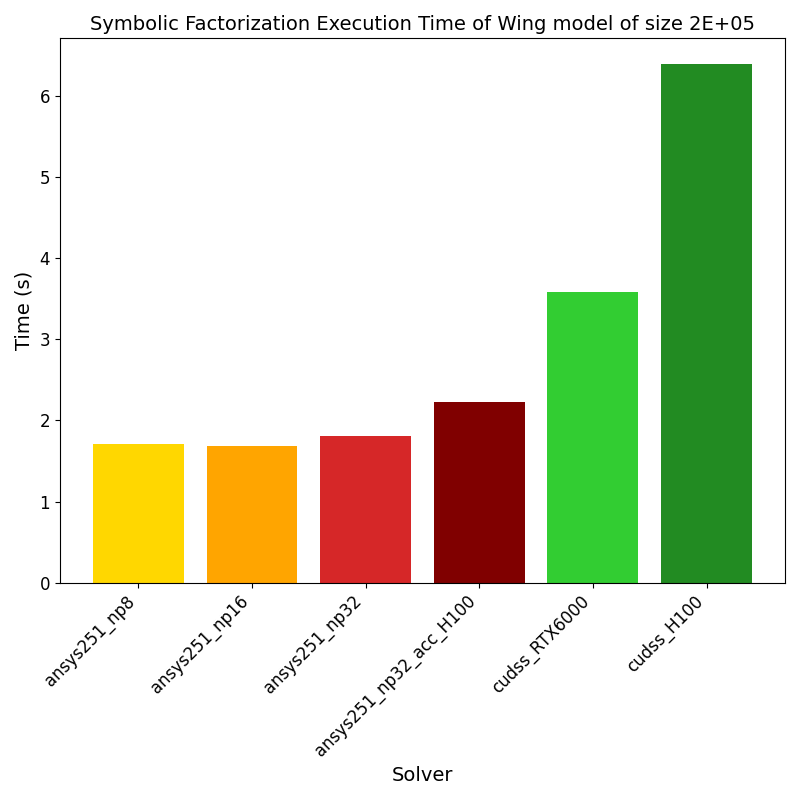
\includegraphics[width=0.49\linewidth]{results/cudss_bench/wing_symbolic_facto_2E5.png}
    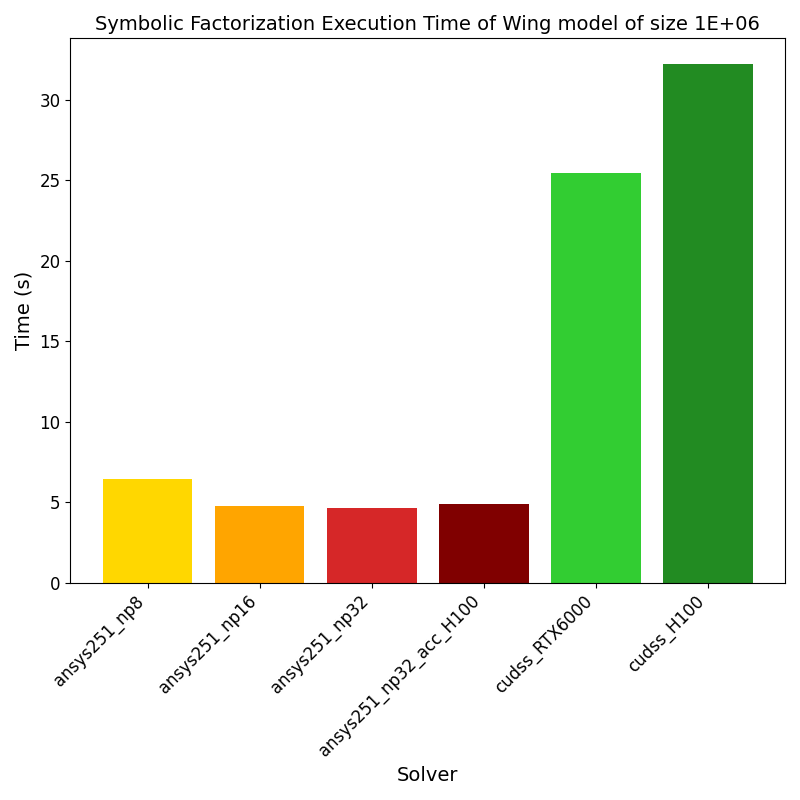
\includegraphics[width=0.49\linewidth]{results/cudss_bench/wing_symbolic_facto_1E6.png}
    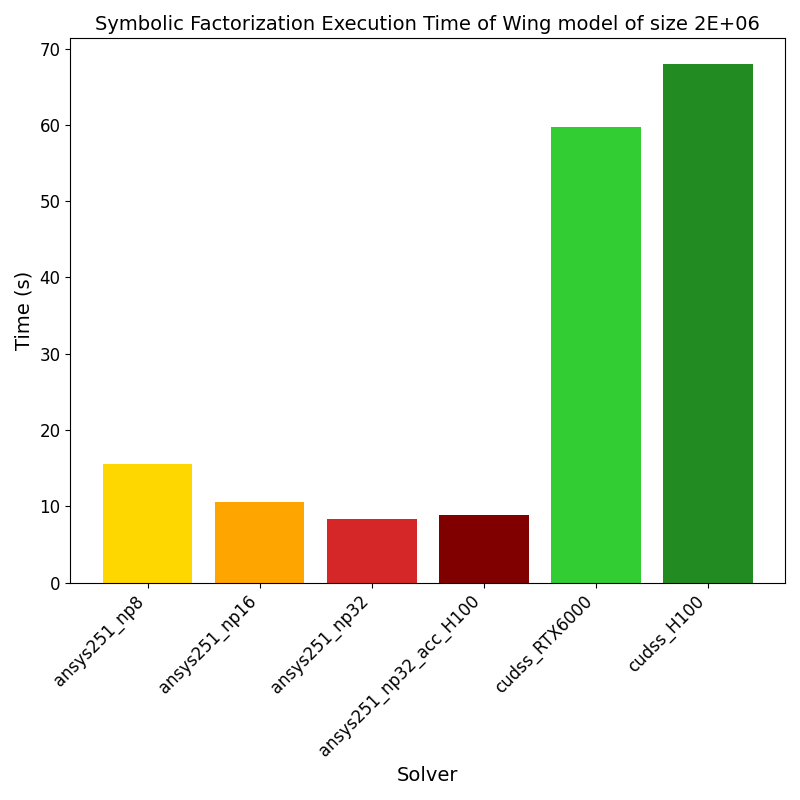
\includegraphics[width=0.49\linewidth]{results/cudss_bench/wing_symbolic_facto_2E6.png}
    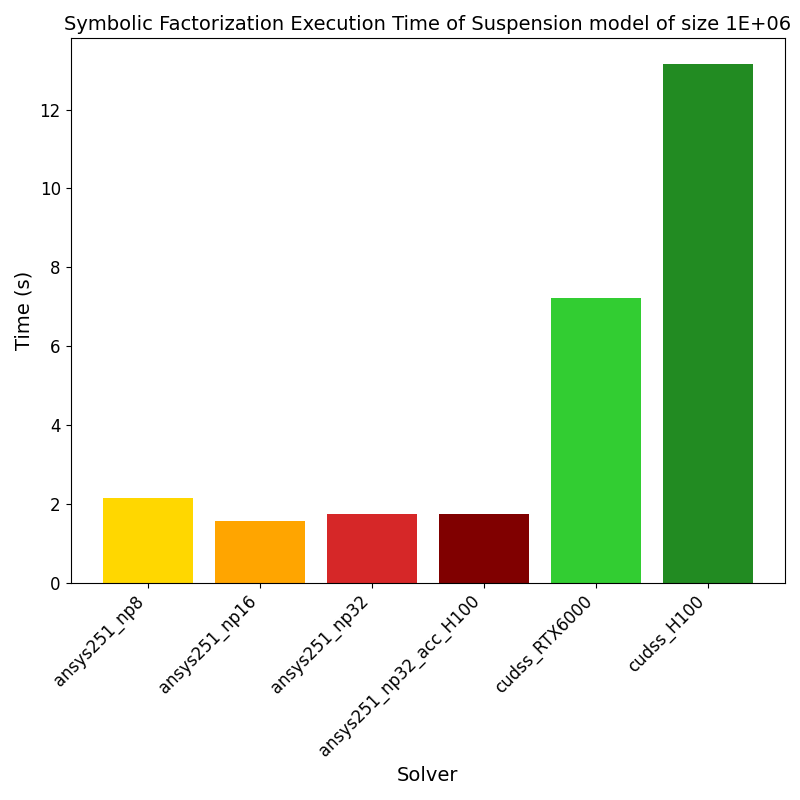
\includegraphics[width=0.49\linewidth]{results/cudss_bench/suspension_symbolic_facto_1E6.png}
    \caption{Symbolic Factorization benchmark results}
    \label{fig:cudss_symbo}
\end{figure}

\begin{figure}[H]
    \centering
    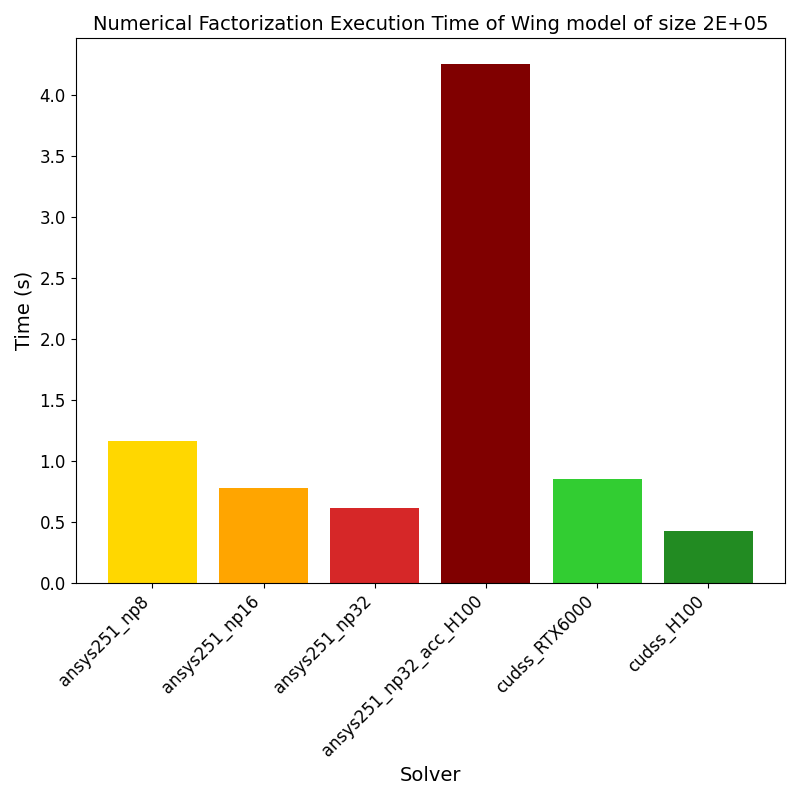
\includegraphics[width=0.49\linewidth]{results/cudss_bench/wing_numerical_facto_2E5.png}
    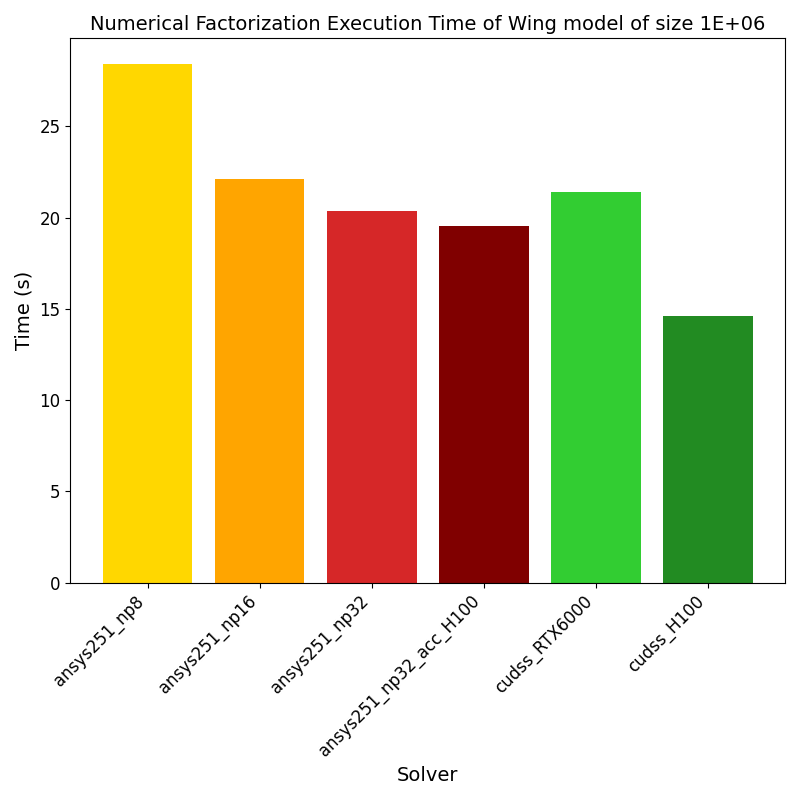
\includegraphics[width=0.49\linewidth]{results/cudss_bench/wing_numerical_facto_1E6.png}
    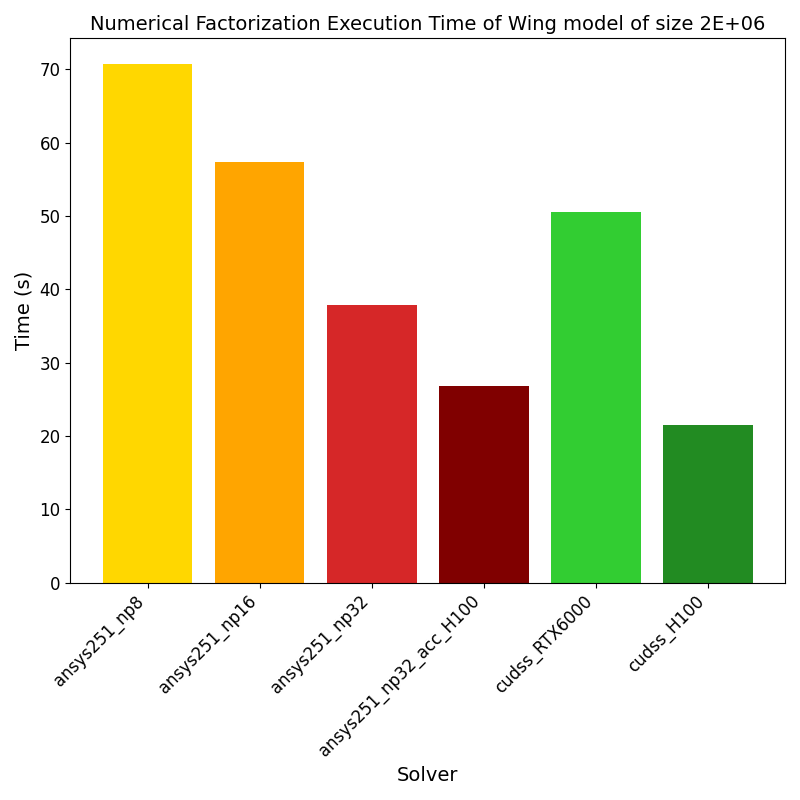
\includegraphics[width=0.49\linewidth]{results/cudss_bench/wing_numerical_facto_2E6.png}
    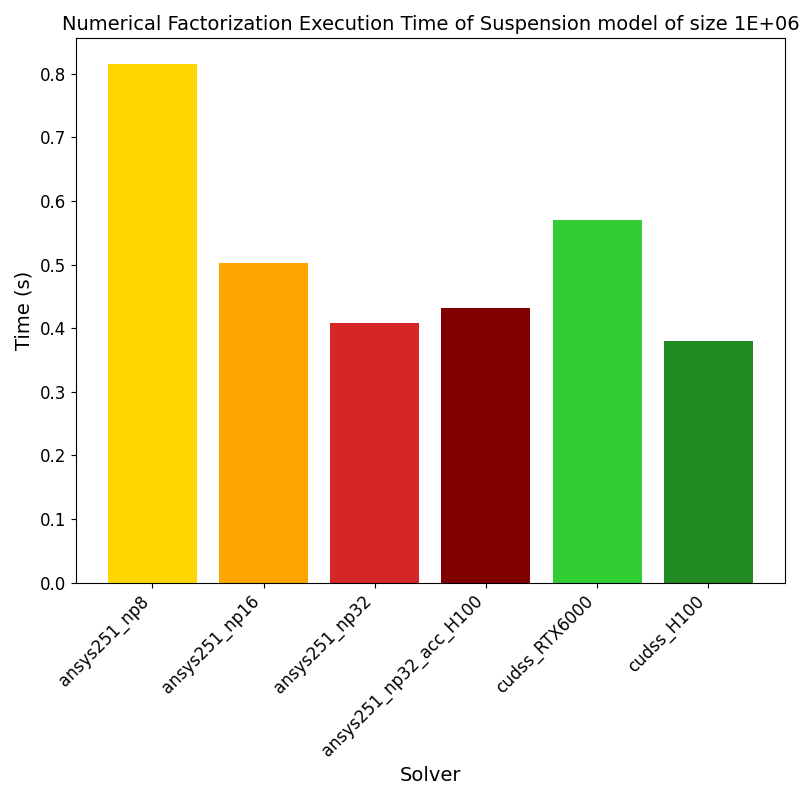
\includegraphics[width=0.49\linewidth]{results/cudss_bench/suspension_numerical_facto_1E6.png}
    \caption{Numerical Factorization benchmark results}
    \label{fig:cudss_num}
\end{figure}

\begin{figure}[H]
    \centering
    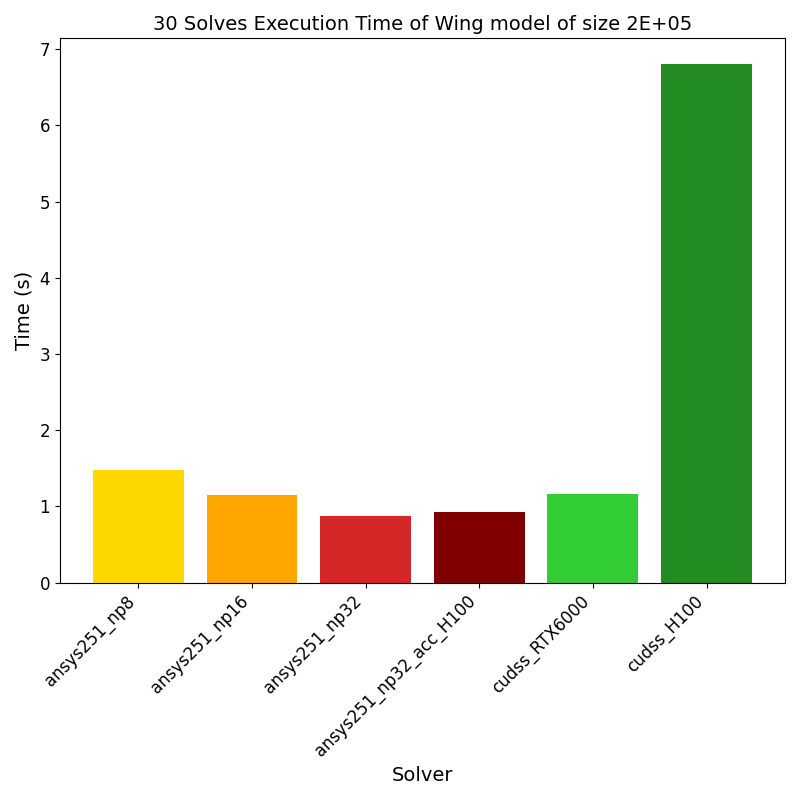
\includegraphics[width=0.49\linewidth]{results/cudss_bench/wing_solve_2E5.png}
    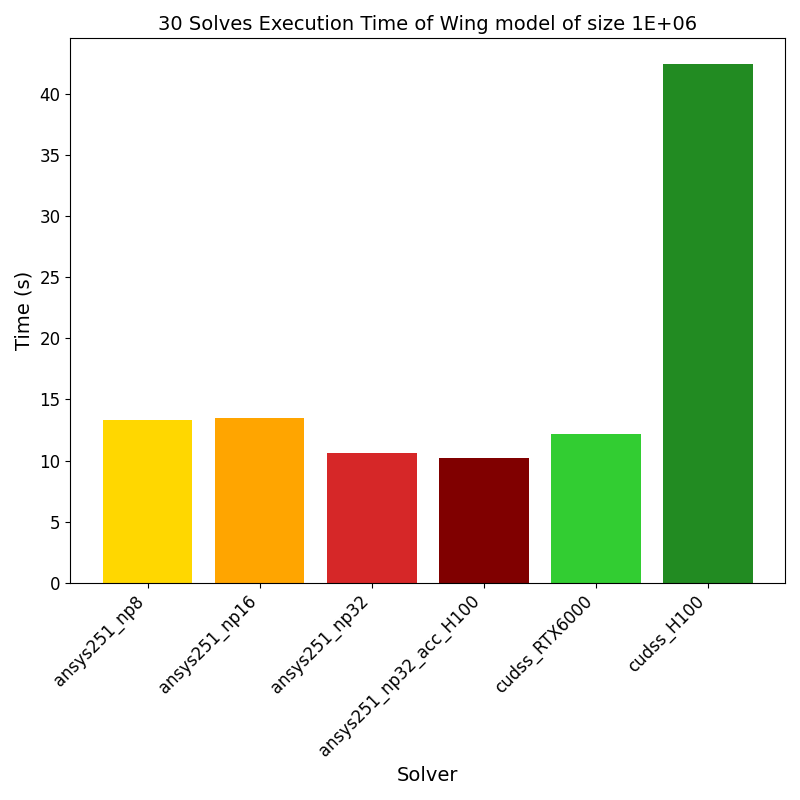
\includegraphics[width=0.49\linewidth]{results/cudss_bench/wing_solve_1E6.png}
    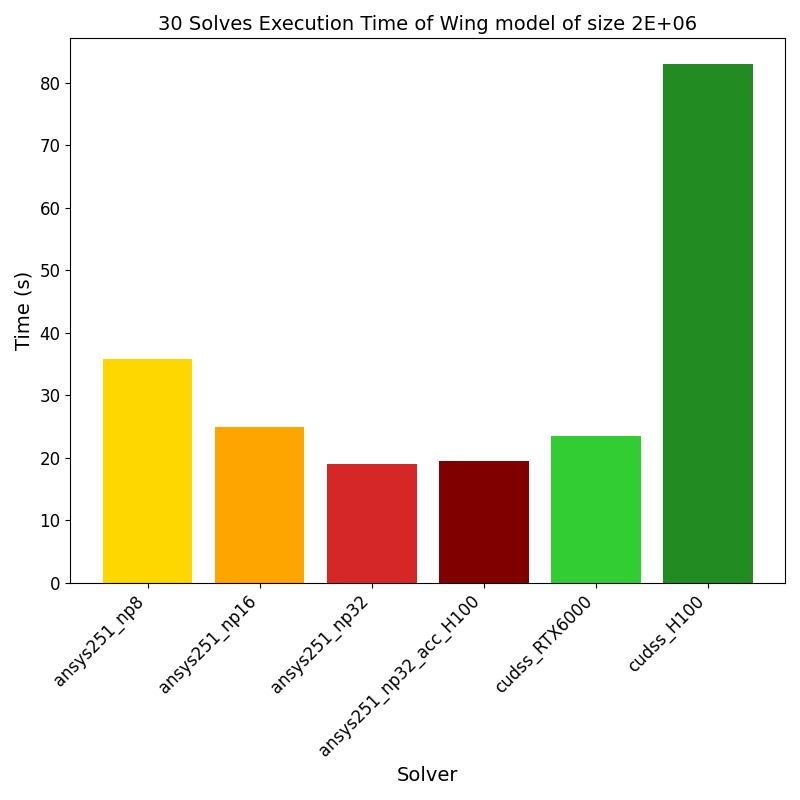
\includegraphics[width=0.49\linewidth]{results/cudss_bench/wing_solve_2E6.png}
    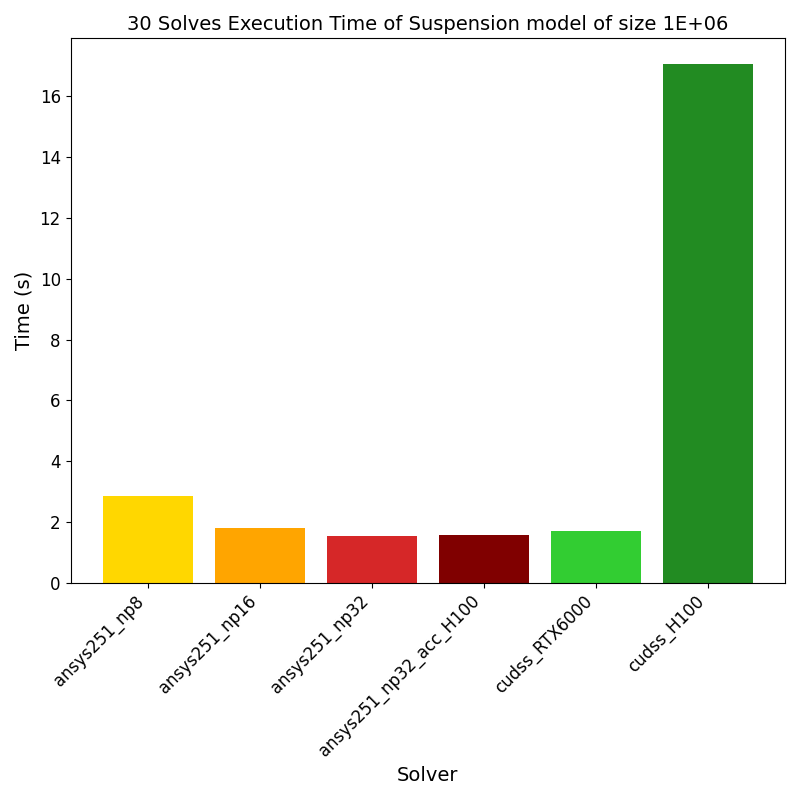
\includegraphics[width=0.49\linewidth]{results/cudss_bench/suspension_solve_1E6.png}
    \caption{Solve benchmark results}
    \label{fig:cudss_solve}
\end{figure}


\paragraph*{}
Since we only requested 50 eigenfrequencies, no shifting was necessary during the solve process. Only one symbolic factorization and one numerical factorization were required. The algorithm needed 30 iterations to capture the 50 eigenfrequencies, resulting in the solution of 30 linear systems. The benchmark results are grouped according to the solve phase. The figure \ref{fig:cudss_symbo} shows the symbolic factorization results, figure \ref{fig:cudss_num} shows the numerical factorization results and figure \ref{fig:cudss_solve} shows the solve results.

\paragraph*{}
The labels along the $x$ axis denote the solver used to solve the linear system. \texttt{ansys251\_np8} means the Ansys's solver from the release R251 distributed on 8 cores. The \texttt{\_acc\_H100} term means that we enabled the GPU acceleration of the factorization phase (that is not part of our work) on a NVIDIA H100. The \texttt{cudss\_RTX6000} denote the NVIDIA's cuDSS solver running on a NVIDIA RTX 6000 Ada Generation.

\paragraph*{}
Firstly, we observe that both the CPU and GPU solvers scale similarly with the model size. The execution time ratios remain consistent for models of 200,000, 1,000,000, and 2,000,000 units. However, GPU acceleration for numerical factorization is only advantageous for model sizes exceeding 1,000,000.

\paragraph*{}
Secondly, concerning the symbolic factorization phase, Ansys's solver is significantly faster than NVIDIA's one, being up to 6 times quicker depending on the model size. We also notice that this operation is surprisingly faster on NVIDIA RTX6000 Ada generation than on a NVIDIA H100. This outcome is unexpected because the NVIDIA H100 is currently the best GPU available on the market.

\paragraph*{}
Thirdly, regarding numerical factorization, the cuDSS solver running on an NVIDIA H100 is the fastest, although it is nearly matched by the fastest of Ansys. The performance of the cuDSS solver on an NVIDIA RTX6000 Ada generation is comparable to Ansys's performance distributed across 16 cores. This indicates that GPUs significantly impact numerical factorization time, with the operation being faster on an H100 as expected.

\paragraph*{}
Fourthly, regarding the solve execution time, we observe that Ansys distributed on 32 cores is the fastest one. But surprisingly, cuDSS running on a NVIDIA H100 is by far the slowest one, whereas it is closely matching the performances of Ansys distributed on 16 cores with a NVIDIA RTX6000 Ada generation.

\paragraph*{}
Finally, the overall factorization and solve process is faster with Ansys's solver compared to NVIDIA cuDSS, which is good news for Ansys. However, we need to be cautious when analyzing the results, as the performance of the cuDSS solver varies significantly depending on the solve phase and the hardware used. Notably, cuDSS can even perform faster on GPUs with less number of cores.


\newpage
\section{TOAR Algorithm}

\paragraph*{}
As I had finished working on the initial objectives of my internship, we decided to take it a step further and work on implementing an eigensolver for \acrfull{qep}. The new objectives was to implement a GPU version of the \acrfull{toar} algorithm. Let's first introduce some definitions to better understand the algorithm.


\subsection{Second-order Krylov subspace}
\paragraph*{}
Let $A$ and $B$ be $n\times n$ matrices and $\mathbf{r}_{-1}, \mathbf{r}_0$ be length-$n$ vectors such that $[\mathbf{r}_{-1}, \mathbf{r}_0] \neq \mathbf{0}$. Then the sequence $\mathbf{r}_{-1}, \mathbf{r}_{0}, \mathbf{r}_{1},...,$ with
\begin{align}
    \mathbf{r}_{j} = A\mathbf{r}_{j-1} + B\mathbf{r}_{j-2} \text{ for } j\geq 1
\end{align}
is called a \textit{second-order Krylov sequence} based on $A, B, \mathbf{r}_{-1}$ and $\mathbf{r}_{0}$. The subspace
\begin{align}
    \mathcal{G}_k(A,B;\mathbf{r}_{-1},\mathbf{r}_{0}) = \text{span}\{\mathbf{r}_{-1}, \mathbf{r}_{0}, \mathbf{r}_{1},...,\mathbf{r}_{k-1} \}
\end{align}
is called a $k$-th \textit{second-order Krylov subspace}.

\paragraph*{}
The second-order Krylov subspace $\mathcal{G}_k(A,B;\mathbf{r}_{-1},\mathbf{r}_{0})$ can be embedded in the linear Krylov subspace

\begin{align}
\mathcal{K}_k(L, \mathbf{v}_0) & = \text{ span }\{ \mathbf{v}_0, L\mathbf{v}_0,L^2\mathbf{v}_0,...,L^{k-1}\mathbf{v}_0 \} \\
    & =\text{ span } \left\{ 
    \begin{bmatrix} \mathbf{r}_{0} \\ \mathbf{r}_{-1} \end{bmatrix},
    \begin{bmatrix} \mathbf{r}_{1} \\ \mathbf{r}_{0} \end{bmatrix},
    \begin{bmatrix} \mathbf{r}_{2} \\ \mathbf{r}_{1} \end{bmatrix},
    ...,
    \begin{bmatrix} \mathbf{r}_{k-1} \\ \mathbf{r}_{k-2} \end{bmatrix}
    \right\}
\end{align}
where
\begin{align*}
    L = \begin{bmatrix}
        A & B \\
        I & 0
    \end{bmatrix} \in \mathbb{R}^{2n\times 2n} \text{ and } \mathbf{v}_0 = \begin{bmatrix} \mathbf{r}_{0} \\ \mathbf{r}_{-1} \end{bmatrix} \in  \mathbb{R}^{2n}
\end{align*}
and $I$ is an identity matrix of size $n$. Specifically, let $\mathcal{Q}_k$ and $\mathcal{V}_k$ be basis matrices of the subspaces $\mathcal{G}_k(A,B;\mathbf{r}_{-1},\mathbf{r}_{0})$ and $\mathcal{K}_k(L, \mathbf{v}_0)$ respectively. Then
\begin{align}\label{eq:VQU}
    \mathcal{V}_k = \begin{bmatrix} 
        \mathcal{Q}_k\mathcal{U}_k^{[1]} \\
        \mathcal{Q}_k\mathcal{U}_k^{[2]}
    \end{bmatrix} = \begin{bmatrix}
        \mathcal{Q}_k & \\
        & \mathcal{Q}_k
    \end{bmatrix} \begin{bmatrix}
        \mathcal{U}_k^{[1]} \\
        \mathcal{U}_k^{[2]}
    \end{bmatrix} = \mathcal{Q}_{[k]}\mathcal{U}_k
\end{align}
Note that $\mathcal{Q}_k$ is $n\times \eta_k$, $\mathcal{U}_k^{[1]}$ and $\mathcal{U}_k^{[2]}$ are $\eta_k \times k$, where $\eta_k$ is the dimension of $\mathcal{G}_k(A,B;\mathbf{r}_{-1},\mathbf{r}_{0})$. Note also that $\eta_k \le k+1$ due to possible deflations. Equation \eqref{eq:VQU} indicates a memory-efficient compact representation of the basis matrix $\mathcal{V}_k$ since the memory size $2nk$ required to store $\mathcal{V}_k$ is reduced to $(n+2k)\eta_k$ for $\mathcal{Q}_k$ and $\mathcal{U}_k$. 

\subsection{TOAR algorithm}
\paragraph*{}
The \acrshort{toar} algorithm \refalg{alg:toar} compute an orthogonal basis matrix $\mathcal{Q}_k$ of the second-order Krylov subspace $\mathcal{G}_k(A,B;\mathbf{r}_{-1},\mathbf{r}_{0})$ while maintaining the basis matrix $\mathcal{V}_k$ of the associated linear Krylov subspace $\mathcal{K}_k(L, \mathbf{v}_0) $ as orthogonal.

\paragraph*{}
Recall that the Arnoldi procedure computes an orthogonal basis of the $k$-th Krylov subspace $\mathcal{K}_k(L, \mathbf{v}_0) $ such that 
\begin{align}
    \mathcal{H}_k = \mathcal{V}_k^T L \mathcal{V}_k
\end{align}
see equation \eqref{eq:arnoldi} for more details. From equation \eqref{eq:VQU} we have
\begin{align}
    \mathcal{H}_k =
        \begin{bmatrix} 
            \mathcal{Q}_k\mathcal{U}_k^{[1]} \\
            \mathcal{Q}_k\mathcal{U}_k^{[2]}
        \end{bmatrix}^T
        \begin{bmatrix}
            A & B \\
            I & 0
        \end{bmatrix}
        \begin{bmatrix} 
            \mathcal{Q}_k\mathcal{U}_k^{[1]} \\
            \mathcal{Q}_k\mathcal{U}_k^{[2]}
        \end{bmatrix}
\end{align}
The TOAR algorithm computes $\mathcal{Q}_k$, $\mathcal{U}_k^{[1]}$ and $\mathcal{U}_k^{[2]}$ without explicitly generating $\mathcal{V}_k$.

\subsection{Implementation}

 \begin{algorithm}
\caption{Two-level Orthogonal ARnoldi (TOAR) Algorithm}\label{alg:toar}
\begin{algorithmic}[1]
\Require $A,B \in \mathbb{R}^{n \times n} \text{ and } r_{-1}, r_0 \in \mathbb{R}^n \text{ with } \gamma = \lVert [r_{-1},r_0] \rVert_F \neq 0$ and subspace order $k$
\Ensure $\mathcal{Q}_k \in \mathbb{R}^{n \times \eta_k}, \mathcal{U}_{k,1}, \mathcal{U}_{k,2} \in \mathbb{R}^{\eta_k \times k} \text{ and } \mathcal{H}_k = \{h_{ij}\} \in \mathbb{R}^{k\times k-1}$

\State $QX = \mathtt{RRQR}([r_{-1},r_0]) $ with $\eta_1$ being the rank
\State Initialize $\mathcal{Q}_1 = Q, \mathbf{u}_{1}^{[1]} = X_{:,2}/\gamma \text{ and } \mathbf{u}_{1}^{[2]} = X_{:,1}/\gamma$
\For{$j=1,2,...,k-1$}
    \State $\mathbf{r} = A(\mathcal{Q}_j \mathbf{u}_{j}^{[1]}) + B(\mathcal{Q}_j \mathbf{u}_j^{[2]})$
    \For{$i=1,...,\eta_j$} \LineComment{Modified Gram-Schmidt}
        \State $s_i = \mathbf{q}_i^T \mathbf{r}$
        \State $\mathbf{r} = \mathbf{r} - s_i \mathbf{q}_i$
    \EndFor
    \State $\alpha = \lVert \mathbf{r} \rVert_2$
    \State Set $\mathbf{s} = [s_1,...,s_{\eta_j}]^T$

    \For{$i=1,...,j$} \LineComment{Modified Gram-Schmidt}
        \State $h_{ij} = \mathbf{u}_{i}^{[1]T} \mathbf{s} + \mathbf{u}_i^{[2]T} \mathbf{u}_j^{[1]}$
        \State $ \mathbf{s} = \mathbf{s} - h_{ij}\mathbf{u}_i^{[1]}$
        \State $\mathbf{u}_j^{[1]} = \mathbf{u}_j^{[1]} - h_{ij}\mathbf{u}_i^{[2]}$
    \EndFor

    \State $h_{j+1,j} = (\alpha^2 + \lVert \mathbf{s} \rVert_2^2 +\lVert \mathbf{u} \rVert_2^2 )^{1/2}$
    \If{$h_{j+1,j} = 0$} \LineComment{breakdown}
        \State \textbf{stop}
    \EndIf

    \If{$\alpha = 0$} \LineComment{deflation}
        \State $\mathcal{U}_{j+1}^{[1]} = 
            \begin{bmatrix}
                \mathcal{U}_{j}^{[1]} & s/h_{j+1,j}
            \end{bmatrix}$
         $\quad \mathcal{U}_{j+1}^{[2]} =
            \begin{bmatrix}
            \mathcal{U}_{j}^{[2]} & \mathbf{u}_j^{[1]}/h_{j+1,j}
            \end{bmatrix}$
    \Else
        \State $\eta_{j+1} = \eta_j +1$
        \State $\mathcal{Q}_{j+1} = 
            \begin{bmatrix}
                 \mathcal{Q}_j & \mathbf{r}/\alpha 
            \end{bmatrix}$
        \State $\mathcal{U}_{j+1}^{[1]} = 
            \begin{bmatrix}
                \mathcal{U}_{j}^{[1]} & \mathbf{s}/h_{j+1,j} \\
                0  & \alpha / h_{j+1,j}
            \end{bmatrix}$
         $\quad \mathcal{U}_{j+1}^{[2]} = 
            \begin{bmatrix}
                \mathcal{U}_{j}^{[2]} & \mathbf{u}_j^{[1]}/h_{j+1,j} \\
                0  & 0
            \end{bmatrix}$
    \EndIf
\EndFor

\end{algorithmic}
\end{algorithm}

\paragraph*{}
We see that we already have most of the tools to implement this algorithm. Firstly, this algorithm require some basic linear algebra operations most of the time provided by the \acrshort{blas} libraries.

\paragraph*{}
Secondly, we already studied the Gram-Schmidt orthogonalization that is present line 5 and 11. We then rely on our work concerning orthogonalization procedure (see subsection \ref{seq:ortho}). We will also use the fact that for a relatively big problem size, the \cgsi is actually faster than \mgs on GPU.

\paragraph*{}
Thirdly, The \texttt{RRQR()} subroutines is the \acrlong{rrqr} which is basically a QR factorization that also return the rank of the resulting matrix $R$. This operation can easily be implemented with Gram-Schmidt algorithm.

\paragraph*{}
Finally, at line 4, we solve a linear system in order to implicitly compute the result of the matrix-vector product with $A$ and $B$ since these matrices are implicitly given by $A=-K^{-1}C$ and $B=-K^{-1}M$ (see equation \eqref{eq:implicit_mv}). We will use the cuDSS linear solver that we tested previously (see section \ref{seq:cudss}).

\subsection{Shifting the QEP}
As we did with the generalized eigenvalue problem \eqref{eq:shift}, we can shift the the quadratic eigenvalue problem. Therefore, instead of computing $A=-K^{-1}C$ and $B=-K^{-1}M$, we compute $A = -(\sigma^2 M + \sigma C + K)^{-1} M$ and $B = -(\sigma^2 M + \sigma C + K)^{-1} C$ for a given shift $\sigma$.

\paragraph*{}
I did not have sufficient time to fully implement the method described in \eqref{eq:shift}. We managed to complete only the first step, which involves computing the reduced subspace using the TOAR algorithm. Evaluating the performance of the algorithm is not straightforward because we are unable to compute the final eigenvalues. However, since the TOAR algorithm is supposed to generate an orthogonal subspace $\mathcal{Q}_k$, we can at least measure its orthogonality. The following table presents the results for various problems:

\begin{figure}[h]
\begin{center}
\begin{tabular}{ |c|c|c| } 
 \hline
 Problem size & Subspace size $\eta$ & $\lVert I_{\eta} - \hat{\mathcal{Q}}_{\eta}^T \hat{\mathcal{Q}_{\eta}} \rVert$ \\ 
 \hline
    $M,C,K \in \mathbb{R}^{10 \times 10}$ & 10 & 6.2e-16 \\
    $M,C,K \in \mathbb{R}^{639 \times 639}$ & 455 & 1.5e-14 \\
    $M,C,K \in \mathbb{R}^{915 \times 915}$ & 7 & 5.1e-16 \\
    $M,C,K \in \mathbb{R}^{1940 \times 1940}$ & 201 & 9.7e-15 \\
 \hline
\end{tabular}
\end{center}
\caption{Results of TOAR algorithm}
\label{tab:gs_bound}
\end{figure}

\paragraph*{}
We can see that the orthogonality of $\mathcal{Q}_{\eta}$ is well preserved. However, we notice that the subspace sizes are much smaller than the original matrices size. This is due to deflation in the TOAR algorithm. This need to be addressed in a future work because the size of the subspace may be not big enough the capture all the desired eigenvalues.

\chapter{Conclusion}
\paragraph*{}
In conclusion, the initial goal of accelerating certain parts of an eigensolver has been achieved. Firstly, we were able to identify a better orthogonalization algorithm on the GPU. The advantages of the GPU enable a faster and more numerically robust procedure. However, this result depends on the GPU used. Next, we tested a direct sparse solver, which proved to be interesting as it is faster for numerical factorization phase when solving the linear system. However, it ultimately turned out to be slower and less numerically robust than Ansys's current solver. Finally, we started developing a new GPU-based eigensolver for quadratic eigenvalue problems. Although not yet fully implemented, it's a good start and will be the subject of future work.

\paragraph*{}
Overall, the work carried out is promising and has generated significant interest among several other teams. The work will be continued in the future. I've met some brilliant people who are experts in their field, and worked on some exciting, cutting-edge topics. I am very proud of the results I achieved and I am very pleased to have explored the field of numerical methods and high-performance computing. This internship has been very enriching for me, both technically and personally.









% template <typename T>
% __global__ void sum_reduction_kernel(const size_t dim, const T *vec, T *result) {
%     T partial_sum = 0.;
%     const size_t lane_id  = threadIdx.x%warpSize; 
%     const size_t warp_id = threadIdx.x/warpSize;
%     __shared__ T warps_partial_sum[32]; // max 32 warps per block

%     if(threadIdx.x+blockIdx.x*blockDim.x==0)
%         *result = 0.;
%     __syncthreads();


%     for (size_t idx=threadIdx.x+blockIdx.x*blockDim.x; idx<dim; idx+=gridDim.x*blockDim.x) {
%         if(idx<dim)
%             partial_sum += vec[idx];
%     }
    
%     partial_sum += __shfl_down_sync(0xffffffff, partial_sum, 16, 32);
%     partial_sum += __shfl_down_sync(0xffff0000, partial_sum,  8, 32);
%     partial_sum += __shfl_down_sync(0xff000000, partial_sum,  4, 32);
%     partial_sum += __shfl_down_sync(0xf0000000, partial_sum,  2, 32);
%     partial_sum += __shfl_down_sync(0xc0000000, partial_sum,  1, 32);

%     if (lane_id==0)
%         warps_partial_sum[warp_id] = partial_sum;

%     __syncthreads();

%     if (warp_id==0) {
%         partial_sum = (threadIdx.x < blockDim.x/warpSize) ? warps_partial_sum[lane_id] : 0.;

%             partial_sum += __shfl_down_sync(0xffffffff, partial_sum, 16, 32);
%             partial_sum += __shfl_down_sync(0xffff0000, partial_sum,  8, 32);
%             partial_sum += __shfl_down_sync(0xff000000, partial_sum,  4, 32);
%             partial_sum += __shfl_down_sync(0xf0000000, partial_sum,  2, 32);
%             partial_sum += __shfl_down_sync(0xc0000000, partial_sum,  1, 32);

%         if (threadIdx.x==0)
%             atomicAdd(result, partial_sum);
%     }
% }